\chapter{Гидрометеорология на яхте}

Успех морского плавания, особенно на парусном судне, в значительной степени зависит от погоды, т.е. от состояния атмосферы у земной поверхности в данный момент и на данном месте. Явления природы, создающие погоду на море, рассматривают две смежные науки: метеорология, изучающая земную атмосферу и происходящие в ней физические явления и процессы, и океанология, исследующая, в частности, физические свойства водной среды (гидросферы).

К основным метеорологическим элементам атмосферы, определяющим ее физическое состояние и процессы, происходящие в ней, относятся: атмосферное давление, температура и влажность воздуха, облачность, осадки, видимость и ветер. В океанологии элементами, так или иначе влияющими на состояние погоды, считаются такие гидрологические явления, как волнение, морские течения (в том числе и приливно\-/отливные), температура, соленость и плотность воды.

В отличие от общей гидрометеорологии, которая занимается изучением перечисленных элементов и их взаимодействия, навигационная гидрометеорология носит более узкий характер. Ее задача \--- помочь мореплавателю разбираться в гидрометеорологической обстановке, уметь ее анализировать, правильно, по инструментальным и визуальным наблюдениям оценивать состояние погоды на ближайшее время и, используя официальные прогнозы по радио, уметь определять ожидаемую погоду по местным признакам.

\section{Атмосферное давление}

Основным элементом при прогнозировании погоды в море можно считать атмосферное давление. Старинная морская поговорка довольно длительно говорит об этом:

\begin{quote}
Если барометра стрелки падение \\
Требует в море вниманья и бдения, \\
То штурман тогда лишь спокойно заснет, \\
Когда он высоко и кверху идет. \\
\end{quote}

Физическая сущность атмосферного давления \--- это вес столба воздуха от верхней границы атмосферы до земной (водной) поверхности. Плотность воздуха постоянно меняется от колебаний температуры и влажности и от давления верхних слоев атмосферы на нижние. Вместе с изменением плотности воздуха меняется его вес и атмосферное давление.

Нормальным атмосферным давлением принято считать массу ртутного столба высотой 760 мм на площади 1~см$^2$, находящейся на уровне Мирового океана (уровне моря), при температуре 0\grC и на широте места 45\gr.

В практике метеорологических наблюдений атмосферное давление измеряется миллиметрами ртутного столба, или миллибарами (мбар). Специальные таблицы для перевода единиц атмосферного давления имеются в <<Мореходных таблицах>> (МТ-75).

Для измерения давления в судовых условиях применяют два прибора \--- барометр\-/анероид и барограф.

Шкала \textbf{анероида} (рис.~\ris{109}) градуирована в миллиметрах ртутного столба, а в последние годы \--- в гектопаскалях (гПа) (по международной системе единиц (СИ) стандартное атмосферное давление составляет 1013,247~гПа = 1013,247~мбар = 760~мм~рт.~ст.). На яхте анероид должен храниться в горизонтальном положении.

Показания анероида снимают, не вынимая его из футляра, и исправляют их тремя поправками, которые находят в паспорте прибора:

\begin{enumerate}
\item Поправка шкалы \--- по величине давления. 
\item Поправка на температуру прибора получается при умножении температурного коэффициента <<$c$>> на температуру прибора <<$t$>> по формуле $d = c \cdot t$. 
\item Добавочная поправка \--- на механическое состояние пружины анероида и барокоробки. Эта поправка должна иметь дату определения в паспорте. 
\end{enumerate}

\begin{figure}[htb]
  \centering{}
  \includegraphics[scale=1.2]{0109P}
  \caption{Барометр-анероид}
  \label{fig:109}
  \small
  \centering{}
  1 \--- пружина; 2 \--- анероидная коробка; 3 \--- термометр\-/атташе; 4 \--- отсчет 778,5~мм. 
\end{figure}

Для удобства определения поправки на температуру прибора в анероид включен полукруглый <<термометр\-/атташе>>. Так как поправки анероида могут время от времени изменяться, то перед выходом в плавание его необходимо проверить.

\textbf{Барограф} \--- прибор, ведущий непрерывную запись атмосферного давления на специальной бумажной ленте \--- \textbf{барограмме} (рис.~\ris{110}). Он удобен тем, что позволяет судить oб изменении атмосферного давления во времени, или, как говорят, о \textbf{барометрической} (барической) \textbf{тенденции}. Барабан, на который надевается барограмма, имеет часовой механизм с заводом, при котором лента совершает полный оборот в течение недели. Барограмма имеет сетку, на которой нанесены по горизонтали временные интервалы \--- часы и сутки, а по вертикали \--- давление в миллибарах.

Меняют ленту раз в неделю. При этом на обороте новой барограммы необходимо записывать дату, время начала записи (с точностью до минуты) и координаты яхты. Начало записи должно точно соответствовать моменту записи по судовым часам. В это же время заводят часовой механизм барографа. Держать барограф можно на отдельной полочке или прямо на штурманском столе. В обоих случаях прибор нужно страховать от падения при крене или на волнении. Ставить барограф следует на амортизирующую прокладку (поролон или губчатую резину).

Барометрическую тенденцию (рис.\ris{111}) определяют по характеру кривой на барограмме, как правило, за последние три часа.

\begin{figure*}[htb]
  \centering{}
  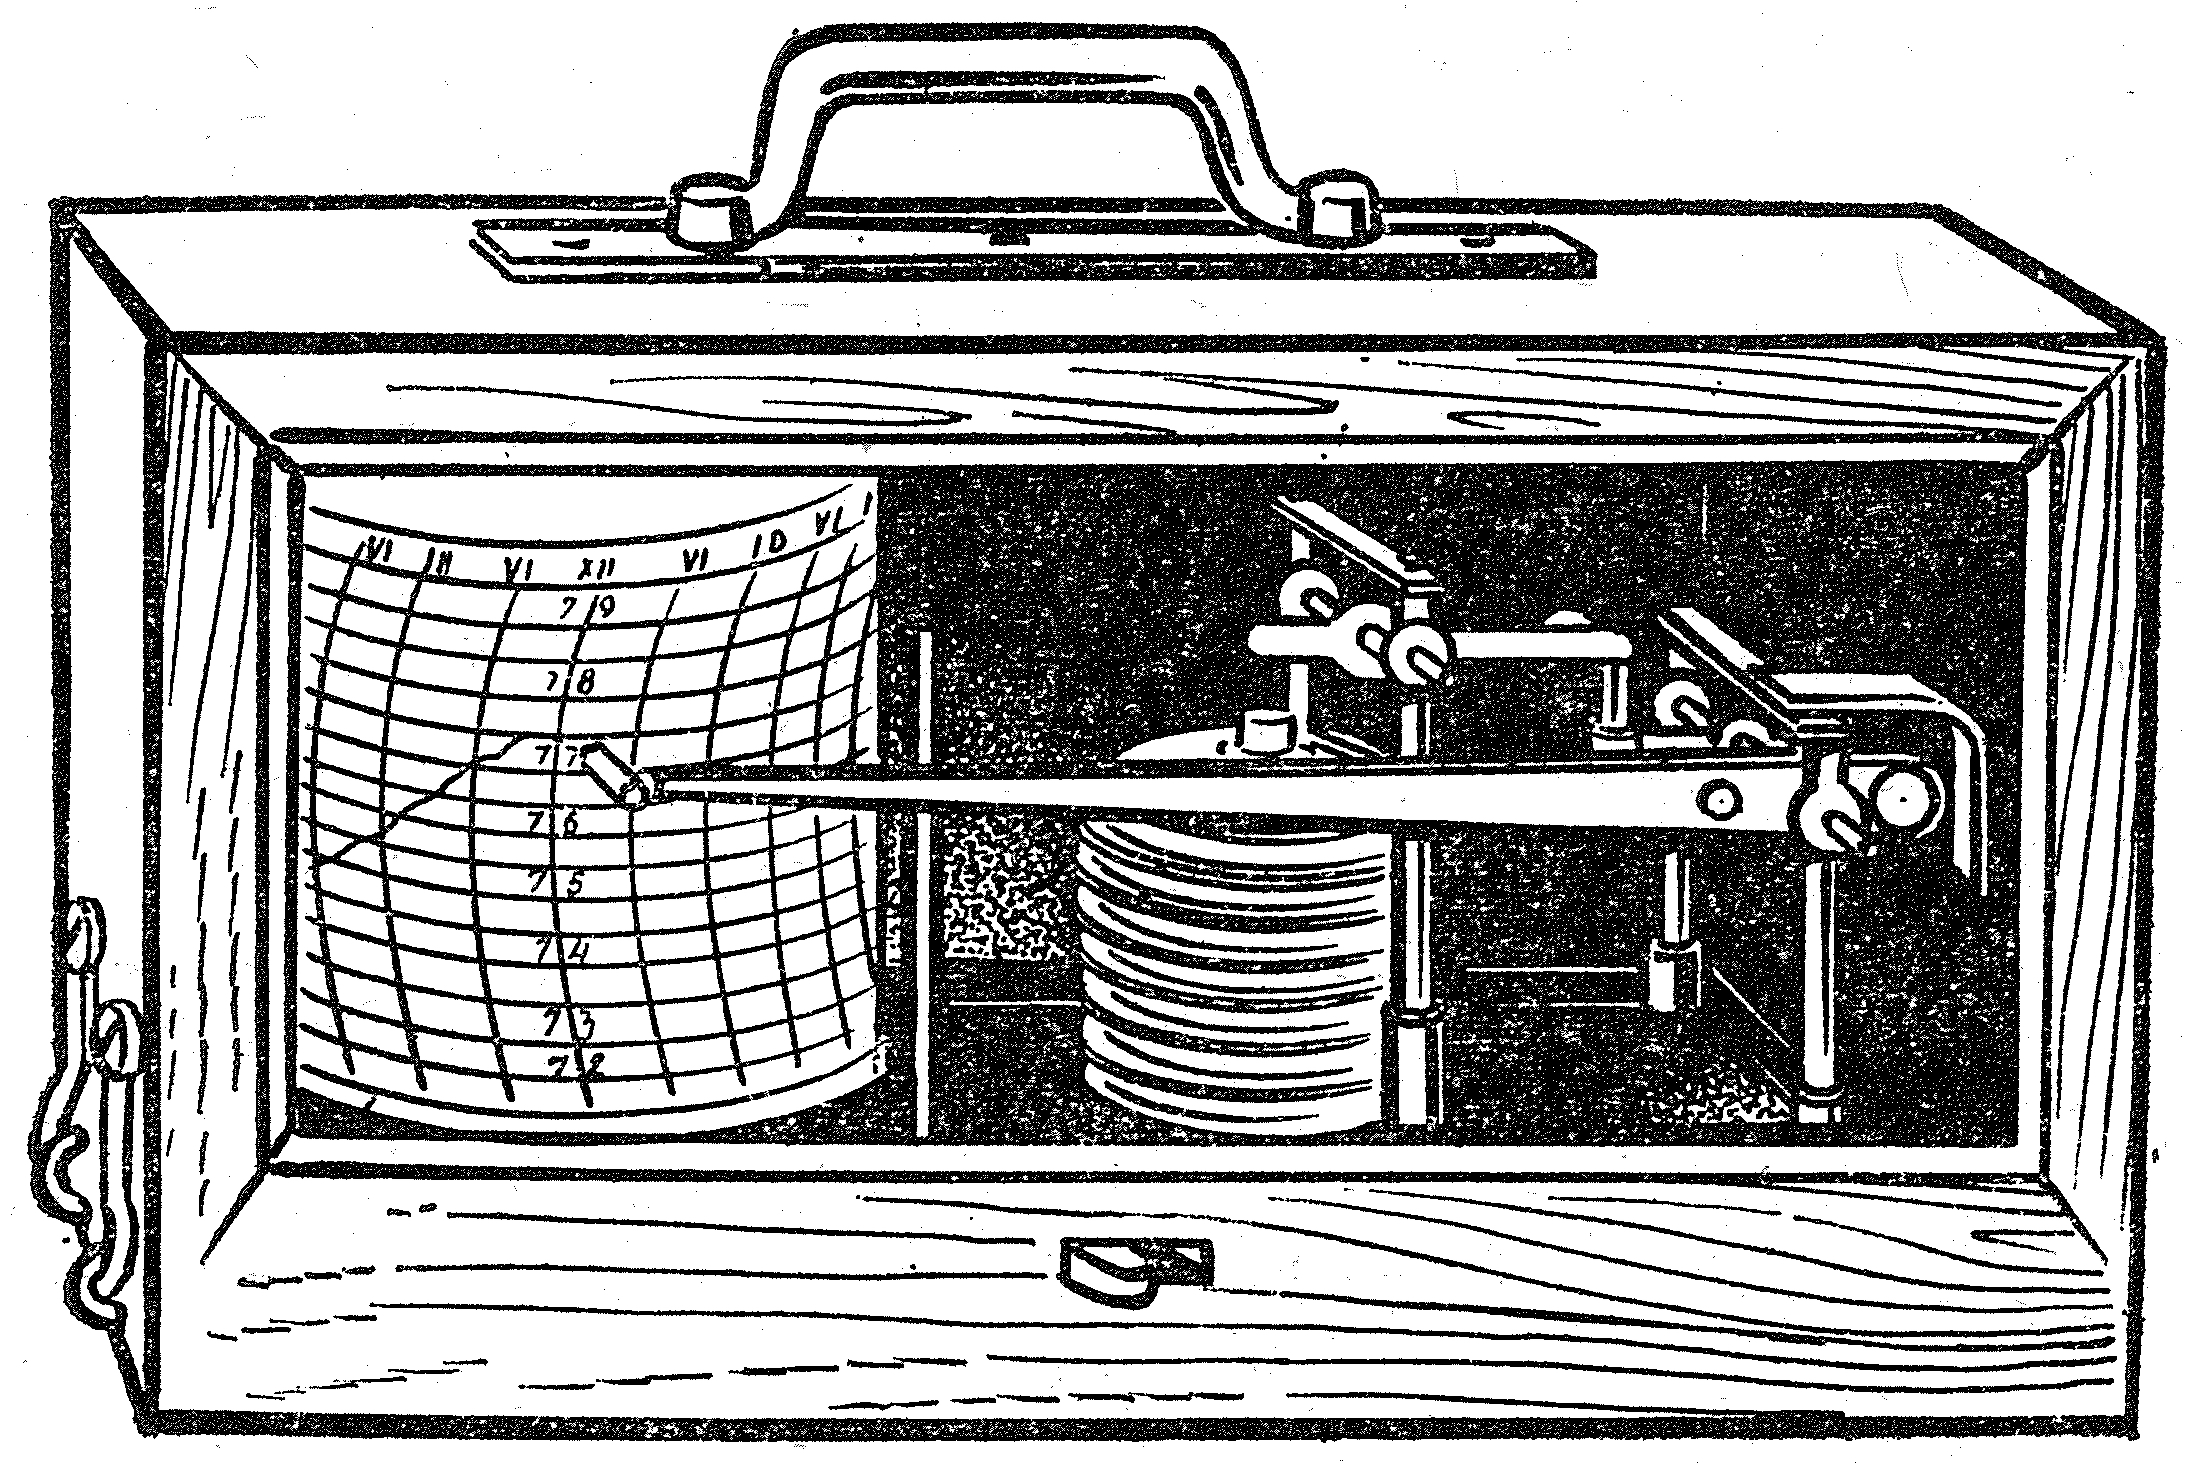
\includegraphics[scale=1.3]{0110P}
  \caption{Барограф \No 4}
  \label{fig:110}
\end{figure*}

\begin{figure*}[htb]
  \centering{}
  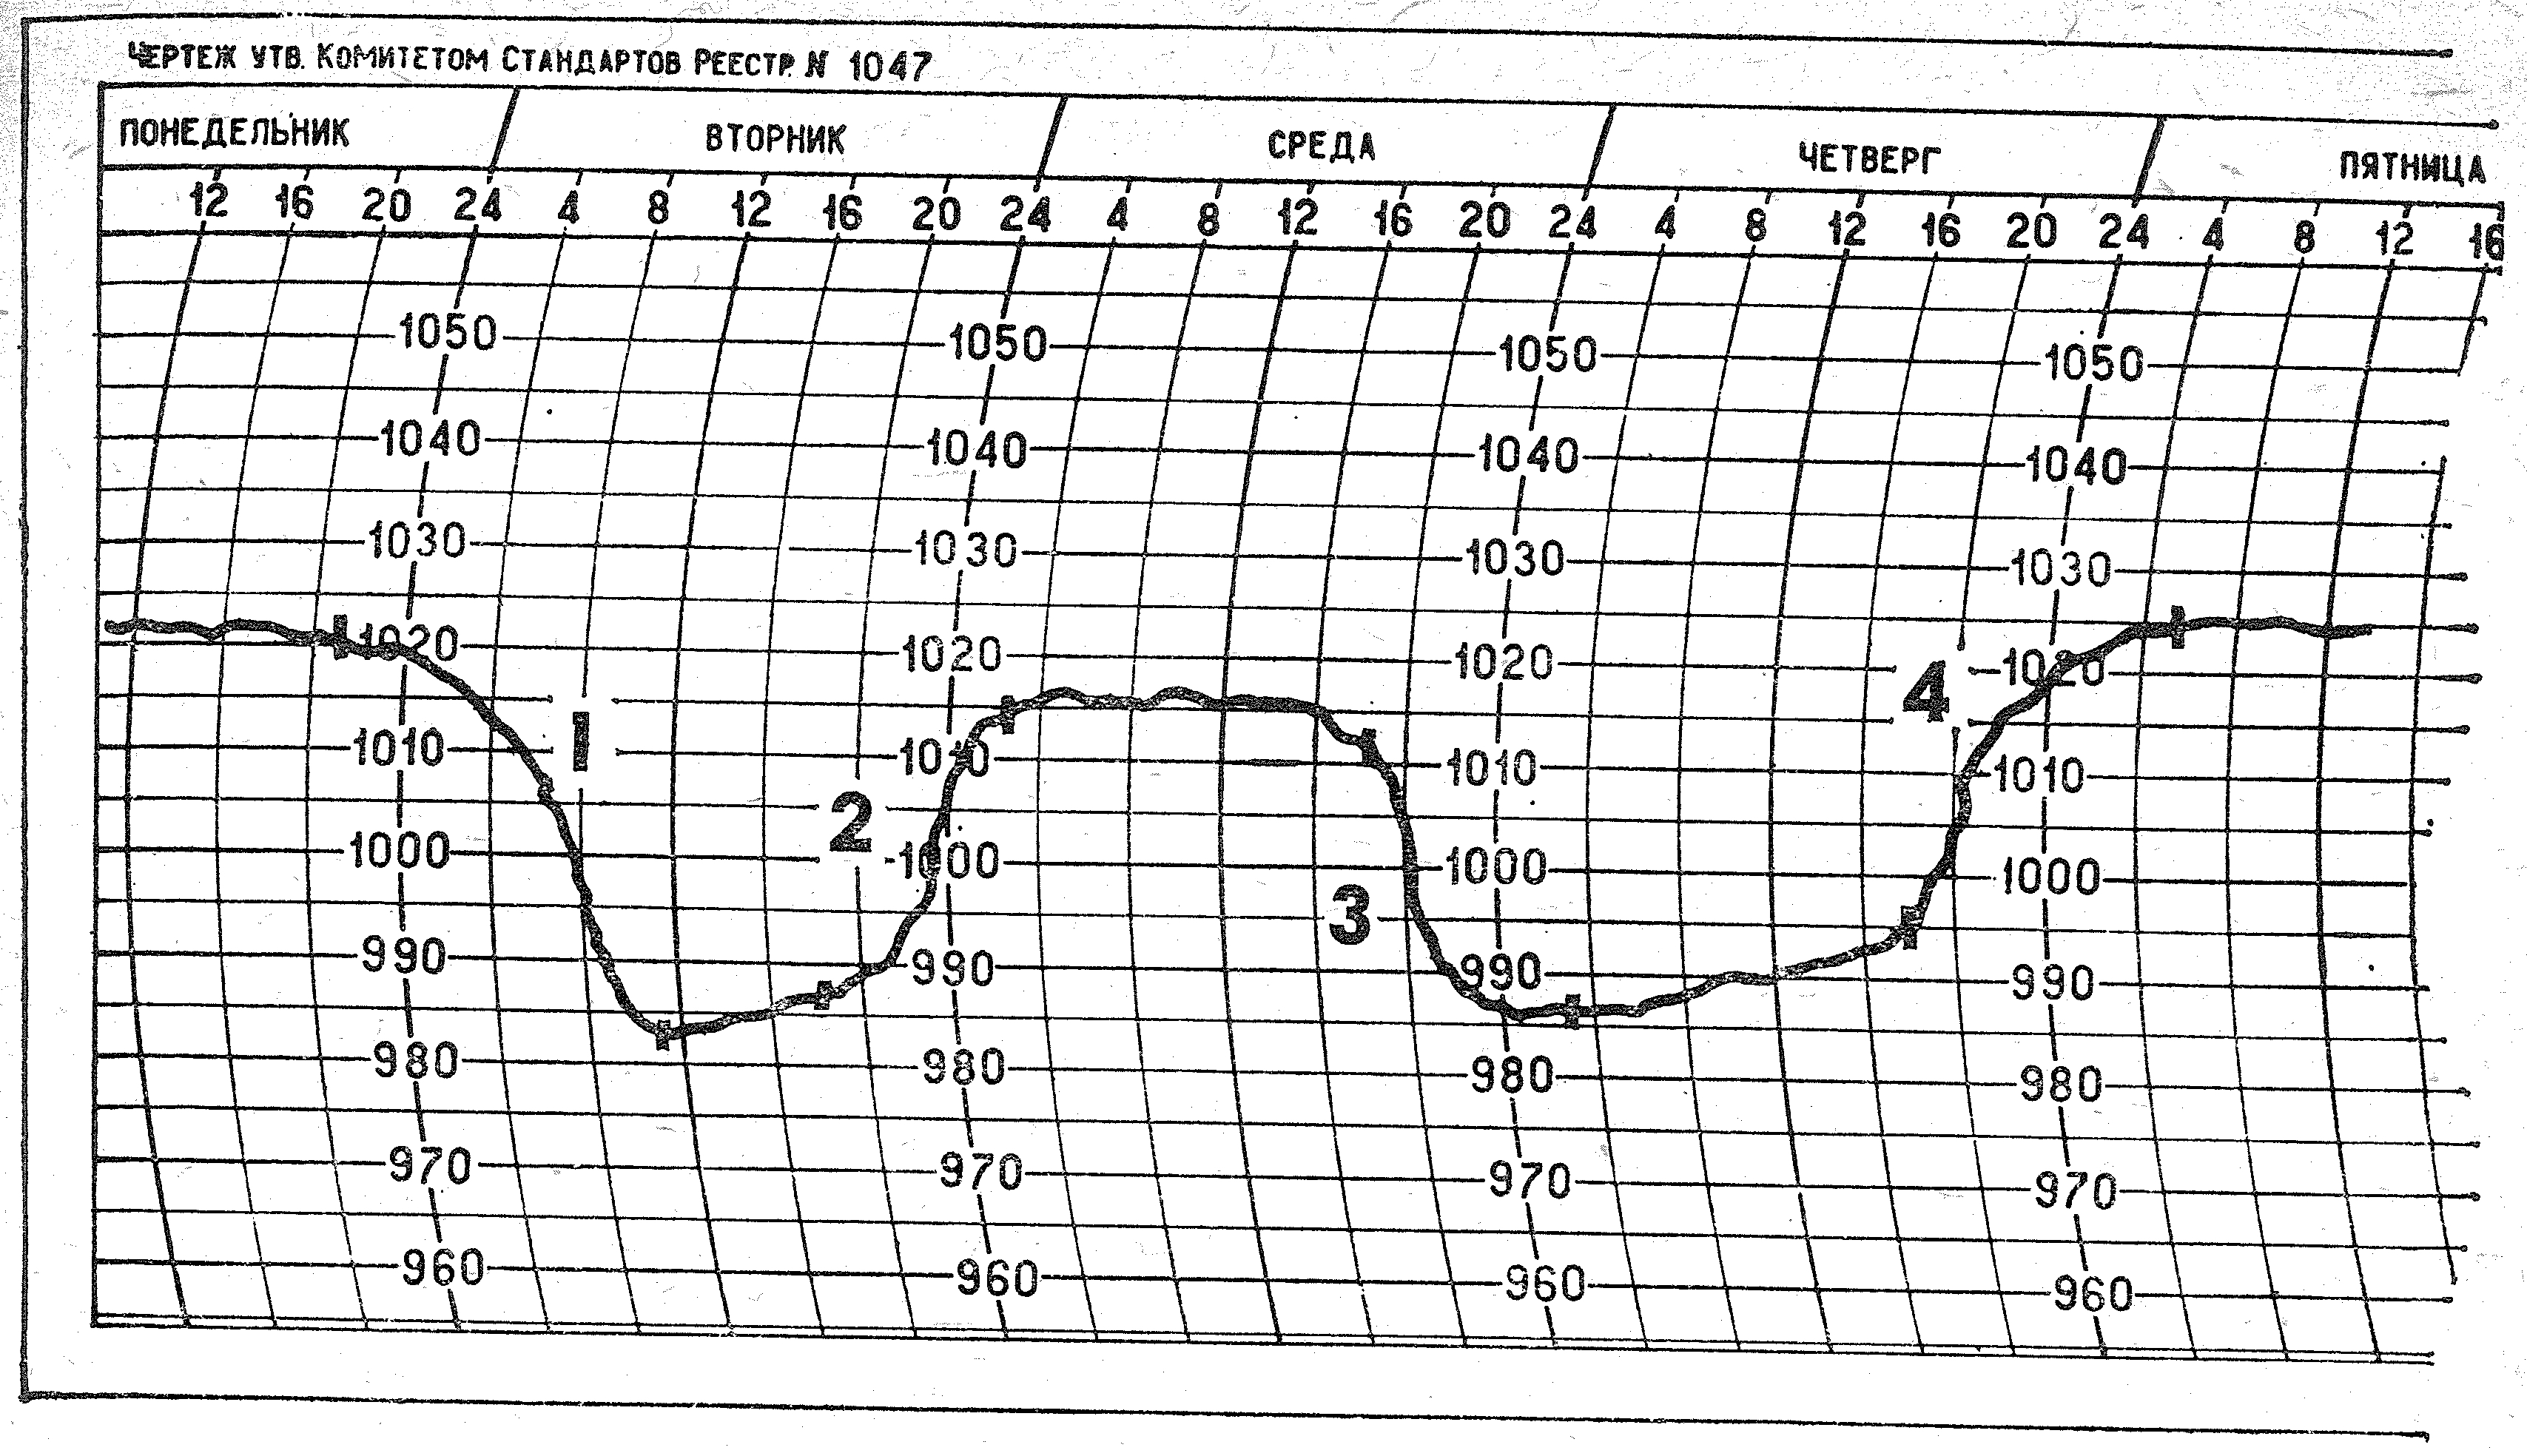
\includegraphics[scale=1.3]{0111P}
  \caption{Примеры барических тенденций}
  \label{fig:111}
  \small
  \centering{}
  Кривая выпуклостью вверх: при падении давления \--- значительное ухудшение погоды (1), при повышении \--- к улучшению погоды (4). Кривая выпуклостью вниз: при падении давления \--- ослабление ветра, некоторое улучшение погоды (3); при повышении \--- может усилиться ветер (2)
\end{figure*}

В суточном ходе атмосферного давления имеется два максимума \--- около 10 и 22 часов и два минимума \--- около 4 и 16 часов.

Показания барометра обычно записывают в судовой журнал при смене вахт, а при неустойчивой погоде \--- не реже чем через 2 часа. В последнем случае давление надо наблюдать чаще и при резком изменении его падения запись делается сразу же.

На справочных или синоптических картах точки с одинаковым атмосферным давлением соединены сплошными линиями \--- изобарами. Все нанесенные на карту изобары составляют барическое поле данного района. Отдельные участки барического поля, отличающиеся своей конфигурацией и типичной разностью давлений, называют барическими системами \--- областями с замкнутыми или незамкнутыми изобарами, с повышенным или пониженным атмосферным давлением.

Различают две замкнутые (основные) барические системы:

\begin{description}
\item[циклон] (барический минимум) \--- область, ограниченная концентрически замкнутыми изобарами, давление в которой понижается от периферии к центру, где наблюдается самое низкое давление (в умеренных широтах \--- 990\otdo 1005~мбар); 
\item[антициклон] (барический максимум) \--- область, также ограниченная изобарами, но отличающаяся от циклона тем, что высокое атмосферное давление в центре антициклона уменьшается к его периферии. 
\end{description}

Незамкнутые изобары складываются в три барические системы:

\begin{description}
\item[ложбина] \--- область низкого давления, отходящая от циклона; 
\item[гребень] \--- область высокого давления, отходящая от антициклона; 
\item[седловина] \--- барическая система, расположенная крестообразно между соседними двумя циклонами и двумя антициклонами.
\end{description}

\section{Температура воздуха}

Температура воздуха в нижних слоях атмосферы складывается в основном из температуры подстилающей поверхности - земли или воды, получающей основную часть тепловой энергии солнца. Тепло приземных слоев воздуха верхним передается двумя путями:

\begin{itemize}
\item непосредственным вертикальным смешиванием теплых нижних слоев с верхними в результате \textbf{конвекции}, т.\=,е. когда теплый воздух поднимается вверх, а более холодный воздух верхних или соседних слоев заменяет его. Над морем конвекция всегда усиливается ночью, при незначительном изменении температуры воды и более сильном охлаждении верхних слоев воздуха; 
\item вихреобразным, т.\=,е. \textbf{турбулентным}, беспорядочным движением воздушных масс, переносящих тепло в самых различных направлениях. 
\end{itemize}

Температура воздуха зависит и от состояния погоды. При сплошной облачности перепады температуры значительно меньше, чем при ясном небе. Во время дождя и после него температура может понижаться.

Наконец, зависит температура воздуха и от широты местности: в тропиках теплее, чем в умеренных или высоких широтах.

При наблюдении за температурой различают ее суточный и годовой ход.

В спортивном мореплавании практическое значение имеет суточный ход т.\=,е. изменение температуры в течение суток в определенном районе. Обычно суточный ход температуры воздуха над морем достигает минимума через 2\otdo 3 часа после восхода солнца, а максимума \--- к 15\otdo 16 часам. Такой суточный ход характерен лишь для устойчивой хорошей погоды. Нарушается он при теплообменных процессах в атмосфере, например при смене теплых воздушных масс холодными. В таких случаях ночная температура может оказаться выше дневной.

\textbf{Суточная амплитуда температуры воздуха} \--- разность между самой высокой и самой низкой температурой за сутки зависит также от облачности, при которой она уменьшается, и от времени года. В открытых морях и океанах суточная амплитуда составляет около 1,0\otdo 1,5\grC, а в закрытых морях может достигать 10\otdo 15\grC. Все это необходимо учитывать, так как характер суточного хода имеет прямое отношение к погоде. Так, нарушение правильного суточного хода температуры предвещает ухудшение погоды, а при резком понижении дневной температуры после ненастья можно ждать улучшения погоды. Ухудшение погоды может наступить и при повышении температуры к вечеру.

\section{Влажность воздуха, облачность, осадки}

Источником влаги в воздухе является вода, испаряющаяся с подстилающей поверхности океанов, морей, озер, рек, водохранилищ. Эта влага находится в атмосфере в трех состояниях: газообразном \--- в виде пара, жидком \--- в виде разной величины капель и твердом \--- в виде снега, града и других ледяных образований. Поскольку водяной пар \--- составная часть атмосферы, он существенно влияет на все атмосферные процессы.

Влажность воздуха определяется наличием в нем водяного пара, и зависит она от количества его массы, в метеорологии учитывают два вида влажности: абсолютную, выраженную массой водяного пара, содержащегося в единице объема воздуха (кг/м$^3$), и относительную, выраженную отношением абсолютной влажности к ее максимальному значению при данной температуре. При 100\,\% относительной влажности в воздухе может произойти конденсация водяных паров с выпадением воды. Температура, при которой это случается, называется точкой росы.

Наглядный пример жидкого и твердого состояния влаги в атмосфере \--- облака, состоящие из мельчайших капелек воды, кристалликов льда или их смеси. Необходимое условие образования облаков \--- насыщение водяных паров до состояния \textbf{конденсации} (превращение пара в воду) или \textbf{сублимации} (превращение пара в ледяные кристаллы, минуя жидкую фазу) и понижение температуры воздуха до критической. Кроме того, в воздухе должны находиться так называемые \textbf{ядра конденсации} (или сублимации). Основная масса ядер конденсации состоит из частиц соли, попавших в атмосферу из испаряющихся водной пыли и брызг во время штормов. Взвешенные в воздухе частицы соли переносятся воздушными потоками до встречи с водяными капельками. Ядрами конденсации могут быть и микроскопические частицы пыли и дымообразующих веществ. Переохлажденные капельки с ядер конденсации, замерзающие при низких температурах, могут сублимироваться и образовывать ледяные кристаллики.

В основу классификации облачных структур взяты латинские слова, характеризующие их внешний вид: страдус (\textit{stratus}) - слой, кумулюс (\textit{cumulus}) - куча, циррус (\textit{cirrus}) - перо, альтус (\textit{altus}) - высокий, опакус (\textit{opakus}) - плотный, нимбус (\textit{nimbus})- дождь, транслюцидус (\textit{translucidus}) - просвечивающий, фрактус (\textit{fractus}) - разорванный, хумилис (\textit{humilis}) - низкий. 

\begin{figure}
  \begin{minipage}[b]{0.49\textwidth}
    \centering
    \includegraphics[scale=1.2]{0112P}
    \caption{Кучевые облака хорошей погоды}
    \label{fig:112}
  \end{minipage}
  \hfil\hfil
  \begin{minipage}[b]{0.49\textwidth}
    \centering
    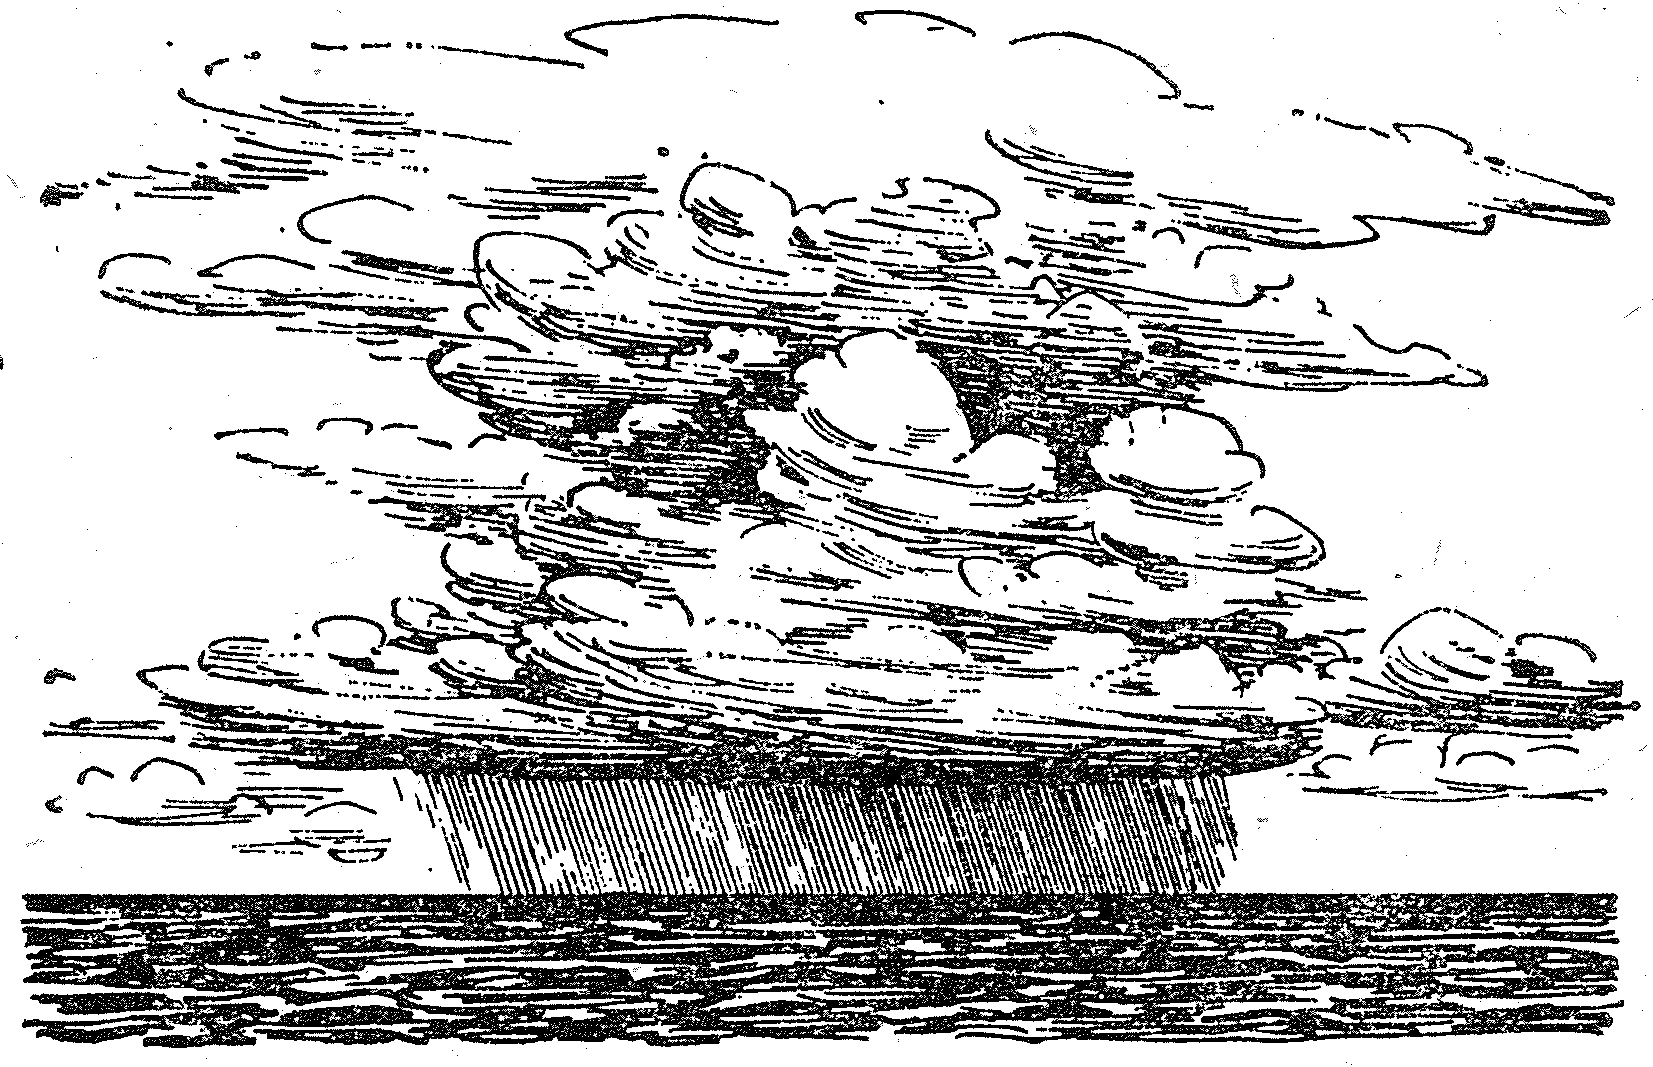
\includegraphics[scale=1.2]{0113P}
    \caption{Кучево-дождевое облако (<<наковальня>>)}
    \label{fig:113}
  \end{minipage}
  \par
  \smallskip
  \begin{minipage}[b]{0.49\textwidth}
    \centering
    \includegraphics[scale=1.2]{0114P}
    \caption{Высококучевые облака (<<барашки>>)}
    \label{fig:114}
  \end{minipage}
  \hfil\hfil
  \begin{minipage}[b]{0.49\textwidth}
    \centering
    \includegraphics[scale=1.2]{0115P}
    \caption{Перистые облака}
    \label{fig:115}
  \end{minipage}
\end{figure}


Классификация выглядит следующим образом:

\begin{enumerate}[I.]
\item Облака нижнего яруса.
  \begin{enumerate}[1)]
  \item Слоистые облака (стратус \--- \textit{St}) \--- высота 0,05\otdo 0,5~км. Сплошной, однородный, серый, низконависающий покров. Обычно дают моросящие осадки. В отдельных случаях могут простираться до видимого горизонта.
  \item Слоисто\-/кучевые (стратокумулюс \--- \textit{Sc}) \--- высота нижнего края 0,3\otdo 1,5~км. Сплошной волнистообразный серый покров, перемежающийся волнами и более светлыми промежутками между ними (\textit{Sc opacus}). Выше 0,6~км образуются слоисто\-/кучевые просвечивающие облака (\textit{Sc translucidus}) серого цвета с просветами. Могут давать морось.
  \item Слоисто\-/дождевые (нимбостратус \--- \textit{Ns}) \--- высота 0,1\otdo 1,0~км. Похожи на слоистые, но имеют более темный цвет. Сопровождаются обложными осадками.
  \item Разорванно\-/слоистые (фрактостратус \--- \textit{Fs}) \--- сильно изорванные слоистые с просветами.
  \end{enumerate}
\itemОблака вертикального развития.
  \begin{enumerate}[1)]
  \item Кучевые облака (кумулюс \--- \textit{Сu}) \--- высота от 0,3 до 1,5~км. Белые кучи с серым плоским основанием и белыми кучеобразными вершинами. К ним относятся кучевые облака хорошей погоды (кумулехумилис \--- \textit{Сu hum}), разорванно\-/кучевые (фрактокумулюс \--- \textit{Fa сu}) и мощные кучевые (кумулюс конгестус \--- \textit{Сu cong}). Эти облака осадков не дают (рис.~\ris{112}).
  \item Кучево\-/дождевые (кумуленимбус \--- \textit{Сb}) \--- вершинами достигают высоты перистых облаков (6\otdo 10~км), походят на горы или высокие башни. Темное основание лежит на высоте около 0,5~км. Вершины ярко\-/белые, состоят из ледяных кристаликов. Верхняя часть облака обычно размыта в стороны, имеет вид наковальни. Эти облака несут сильные ливневые осадки, грозы, град, сопровождаются шквалами (рис.~\ris{113}).
  \end{enumerate}
\item Облака среднего яруса.
  \begin{enumerate}[1)]
  \item Высококучевые (альтокумулюс \--- \textit{Ас}) \--- образуются на высоте 2\otdo 6~км, имеют вид светлых слоисто\-/кучевых просвечивающих облаков в сочетании с параллельными полосами пластинообразных и хлопьевых образований, параллельных гряд, осадков не дают (рис.~\ris{114}).
  \item Высокослоистые (альтостратус \--- \textit{As}) \--- образуются на высоте 3\otdo 5 км в виде пелены светло\-/серого или синеватого цвета. Могут быть просвечивающимися и плотные, создающие пасмурность.
  \end{enumerate}
  Все облака среднего яруса имеют смешанную структуру из смеси капелек с ледяными кристаллами. Осадки, выпадающие из них летом, поверхности земли не достигают.
\item Облака верхнего яруса. 
  \begin{enumerate}[1)]
  \item Перистые (циррус \--- \textit{Ci}) \--- легкие, волокнисто\-/нитевидной формы в виде белых отдельных волокон, иногда <<коготков>> (рис.~\ris{115}).
  \item  Перисто\-/кучевые (циррокумулюс \--- \textit{Сс}) - мелкие <<барашки>>, иногда похожие на рыбью чешую. Могут наблюдаться вместе с перистыми облаками.
    \item Перисто\-/слоистые (цирростратус \--- \textit{Cs}) \--- тонкая белесая прозрачная пелена, на фоне которой вокруг солнца или луны может образоваться ореол из цветных колец, так называемые круги гало. Эти и похожие явления \--- эффект преломления и отражения света в ледяных кристалликах, из которых и состоят перистые облака.
    \end{enumerate}
    Облака верхнего яруса находятся на высоте 6\otdo 10~км.
\end{enumerate}

Конденсат атмосферного водяного пара, выпадающий из облаков или образующийся на поверхности земля и наземных предметах, называется атмосферными осадками, которые могут быть жидкими (дождь, морось; на земле \--- роса) и твердыми (снег, снежная крупа, град; на земле \--- иней, изморозь, гололед).

По своему характеру выпадающие осадки могут быть:

\begin{description}
\item[ливневыми] \--- внезапными и быстротечными выпадениями дождя, снега, крупы или града из кучево\-/дождевых облаков обычно весной и летом;
\item[обложными] \--- продолжительный и равномерный дождь или снег, выпадающий из высокослоистых или слоисто\-/дождевых облаков при пасмурной погоде и на большой площади; в умеренных широтах преобладают осенью и зимой;
\item[моросящими] (морось) \--- мельчайшие капельки воды, не оставляющие следа на воде; выпадают из низких слоистых облаков или из густого тумана; чаще всего бывают осенью. 
\end{description}

Скопление микроскопических капелек воды в нижних слоях атмосферы, при которых горизонтальная видимость составляет менее полумили, называют \textbf{туманом}. Образуются туманы при высокой относительной (около 100\,\%) влажности и в присутствии в воздухе ядер конденсации. По причинам, их вызывающим, туманы делятся на:

\begin{description}
\item[радиационные] \--- возникающие над сушей в предутренние часы из-за потери тепла подстилающей поверхностью.

С повышением дневной температуры быстро рассеиваются. Для мореплавателя такие туманы, лежащие низко над землей (поземные), опасны тем, что, появляясь на побережье, могут закрывать плавучие и береговые знаки навигационного ограждения. При этом могут быть видимы высоко расположенные верхние части зданий, маяков, других береговых предметов. Над морем радиационные туманы появляются только в высоких широтах при большой относительной влажности воздуха; 
\item[адвентивные] (адвекция (лат.) \--- перенос), образующиеся на воде при перемещении теплого влажного воздуха над охлажденной поверхностью моря. Плотны и устойчивы к ветрам до 10~м/с. Перемещаясь с ветром, они заволакивают большие районы. Видимость в адвективных туманах охлаждения может быть от нескольких десятков до нескольких метров. Имея большую высоту над уровнем моря, такой туман усложняет плавание, закрывая не только встречные суда, но и огни маяков; 
\item[адвентивные туманы парения] \--- невысокие, до нескольких метров, клубящиеся туманы, возникающие при перемещении холодного воздуха над теплой поверхностью моря. Встречаются при вторжении холодных масс арктического воздуха на незамерзающие моря в холодное время года.
\end{description}

Разновидностью тумана является туманная дымка, видимость при которой 0,5-5 миль. 

Кроме осадков и туманов на ухудшение видимости может влиять \textbf{сухая мгла} \--- механическое помутнение атмосферы, которое встречается в море вблизи берегов при прохождении мимо больших промышленных городов. Мгла состоит из дыма фабричных труб, концентрации в воздухе различных неулавливаемых частиц пыли, выхлопов двигателей автотранспорта, дыма лесных пожаров и т.\=,д. Другой вид мглы образуется в результате сноса ветром с берега (с сухих песчаных равнин и пустынь) в море пыли и мелкого песка. Смесь тумана и мглы называют \textbf{смогом}.

В сухую жаркую погоду в море можно наблюдать явление оптической мутности атмосферы, когда сильные конвективные токи воздуха различной плотности перемешивают его. При этом в неоднородной воздушной среде при разных температуре и давлении резко меняются условия отражения, рассеивания и преломления световых лучей: предметы теряют свою четкость, становятся расплывчатыми искаженными, снижая тем условия видимости.

В отличие от навигационной метеорологическая видимость определяется предельным расстоянием видимости наблюдаемого предмета в условиях данной погоды. Для определения дневной дальности метеорологической видимости существует десятибалльная шкала (табл.~\ref{tab:5}).

\begin{longtable}[c]{l|p{0.2\textwidth}|p{0.3\textwidth}|c}
  \toprule
  Дальность видимости & Характеристика видимости & Условия видимости & Баллы \\
  \midrule
  \endfirsthead
  \toprule
  Дальность видимости & Характеристика видимости & Условия видимости & Баллы \\
  \midrule
  \endhead
  До 1/4 каб. & \multirow{3}{*}{Очень плохая} & Очень сильный туман & 0 \\
  До 1 каб.   & & Сильный туман & 1 \\
  До 2\otdo 3 каб. & & Умеренный туман & 2 \\
  \midrule
  Около 0,5 мили & \multirow{2}{*}{Плохая} & Слабый туман & 3 \\
  От 0,5 до 1 мили & & Очень сильный дождь, умеренная дымка или мгла & 4 \\
  \midrule
  1\otdo 2 мили & \multirow{2}{*}{Средняя} & Сильный дождь, слабая дымка или мгла & 5 \\
  1\otdo 5 миль & & Умеренный дождь & 6 \\
  \midrule
  5\otdo 11 миль & Хорошая & Слабый дождь & 7 \\ 
  \midrule
  11\otdo 27 миль & Очень хорошая & Без осадков & 8 \\ 
  \midrule
  выше 27 миль & Отличная & Совершенно чистый воздух & 9 \\
  \bottomrule
  \caption{Шкала метеорологической видимости (для летнего плавания)}
  \label{tab:5}
\end{longtable}

\section{Ветер. Общая циркуляция атмосферы}

Перемещение масс воздуха из области высокого атмосферного давления в область с низким давлением называется \textbf{ветром}. Скорость ветра определяется величиной барического градиента, т.\=,е. разностью атмосферного давления на установленную единицу расстояния, равную 60 милям (1\gr широты), в сторону падения давления. Поэтому скорость ветра тем больше, чем больше барический градиент. Величину и направление барического градиента на карте изобар показывают в виде вектора перпендикулярного изобаре большего давления, направленного в сторону меньшего давления. Вследствие вращения Земли (под влиянием силы Кориолиса) направление ветра не совпадает с вектором барического градиента, а отклоняется в северном полушарии вправо, в южном \--- влево. В средних широтах это отклонение достигает 60\gr.

\begin{figure}[htb]
  \centering{}
  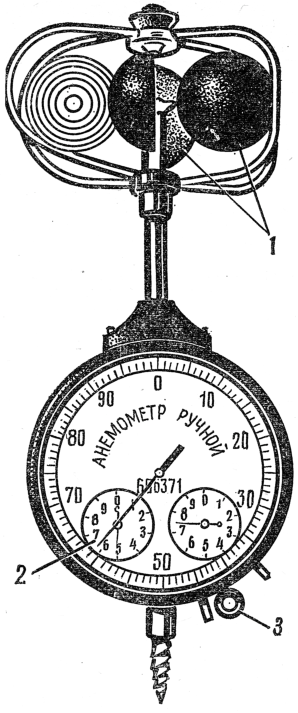
\includegraphics[scale=1.2]{0116P}
  \caption{Ручной анемометр}
  \label{fig:116}
  \small
  \centering{}
  \textit{1} \--- полушария крестовины; \textit{2} \--- отсчет 6175; \textit{3} \--- стопор (арретир)
\end{figure}

На отклонение ветра влияет также кривизна самих изобар, вызывающая криволинейное движение воздуха под действием центробежной силы, направленной по радиусу кривизны. В циклоне центробежная сила направлена против силы градиента, а в антициклоне совпадает с ней. Поэтому при одинаковом градиенте скорость ветра в циклоне всегда меньше, чем в антициклоне.

По традиции направление ветра считается из той точки горизонта, откуда он дует. Иначе говоря, ветер дует в компас, направление обозначается в румбах\footnote{в настоящее время синоним направления} (иногда в градусах). Также в компас принято определять направление зыби, а из компаса, в направлении на горизонт, морские течения.

Единицами измерения скорости ветра являются <<метр в секунду>>, <<километр в час>>, <<узел>>. Практически же скорость ветра с помощью анемометра измеряется в м/с или приближенно оценивается <<сила ветра>> по шкале Бофорта (табл.~\ref{tab:6}).

Для измерения скорости ветра в судовых условиях применяется ручной анемометр (рис.~\ris{116}). Ветер, вращая крестовину с четырьмя полыми полушариями, приводит в движение счетчик прибора, который через три стрелки дает показания на циферблат. Точное значение скорости ветра надо узнать из таблицы поправок в аттестате анемометра.

При порывистом ветре определяют его среднюю скорость \--- по нескольким сделанным подряд измерениям и находят среднее арифметическое значение. Другой способ: проводят наблюдение в течение нескольких минут, а затем делят полученную разность отсчетов на соответствующее число секунд.

Ветер по своей структуре не однороден. Он может быть струйным (ламинарным), когда слои воздуха движутся не перемешиваясь, их частицы не переходят из слоя в сдой. Такое движение воздуха обычно бывает при слабых ветрах. Если же скорость ветра превышает 4~м/с, то частицы воздуха начинают двигаться беспорядочно, его слои перемешиваются и приобретают турбулентный характер. Чем выше скорость ветра, тем больше турбулентность, тем больше скачки скорости в отдельных точках воздушного потока и тем более порывистым становится ветер. Табл.~\ref{tab:7} показывает, как меняется ветер в зависимости от его скорости и направления.

\small
\begin{longtable}{c|c|c|p{0.2\textwidth}|p{0.2\textwidth}|c}
  \toprule
  \multirow{6}{*}{\begin{sideways}\shortstack{Баллы\\Бофорта}\end{sideways}} &
  \multirow{6}{*}{\begin{sideways}\shortstack{Характеристика\\ветра}\end{sideways}} &
  \multirow{6}{*}{\begin{sideways}\shortstack{Скорость ветра\\м/с (интервал)}\end{sideways}} &
  \multicolumn{2}{c|}{Действие ветра} &
  \multirow{6}{*}{\begin{sideways}\shortstack{Давление\\$H/\text{м}^2$}\end{sideways}} \\
  \cmidrule{4-5}
  &\ &\ & \centering{} \multirow{3}{*}{\shortstack{на судне}} & \centering{} \multirow{3}{*}{\shortstack{на море}} & \\
  &\ &\ &\ &\ & \\
  &\ &\ &\ &\ & \\
  &\ &\ &\ &\ & \\
  &\ &\ &\ &\ & \\
  \midrule
  1 & 2 & 3 & \centering{} 4 & \centering{} 5 & 6 \\
  \midrule
  \endfirsthead
  \toprule
  1 & 2 & 3 & \centering{} 4 & \centering{} 5 & 6 \\
  \midrule
  \endhead
  \shortstack{0\\(0)} & Штиль & 0\otdo 0,2 & Дым поднимается вертикально. Вымпел неподвижен & Зеркально-гладкая поверхность & 0 \\
  \midrule
  \shortstack{1\\(1)} & Тихий	& \shortstack{1\\(0,3\otdo 0,5)} & По дыму можно определить направление ветра & Рябь. Пены на гребнях нет & 0,1 \\
  \midrule
  \shortstack{2\\(2)} & Легкий & \shortstack{3\\(1,6\otdo 3,3)} & Легкий поток воздуха. Слегка колеблются флаги и вымпелы & Короткие волны. Гребни кажутся стекловидными & 0,5 \\
  \midrule
  \shortstack{3\\(3)} & Слабый & \shortstack{5\\(3,4\otdo 5,4)} & Дым вытягивается по ветру и развевает флаги и вымпелы & Короткие волны. Гребни образуют стекловидную пену. Изредка образуются маленькие белые барашки & 0,2 \\
  \midrule
  \shortstack{4\\(4)} & Умеренный & \shortstack{7\\(5,5\otdo 7,9)} & Вытягиваются вымпелы, заполаскивают флаги & Удлиненные волны. Белые барашки видны во многих местах & 4 \\
  \midrule
  \shortstack{5\\(4)} & Свежий & \shortstack{9\\(8,0\otdo 10,7)} & Вытягиваются и полощут большие флаги & Развитые в длину, но не крупные волны. Повсюду видны барашки. Отдельные брызги & 6 \\
  \midrule
  \shortstack{6\\(5)} & Сильный & \shortstack{12\\(10,8\otdo 13,8)} & Начинают гудеть провода и снасти & Образуются крупные волны. Белые пенистые гребни занимают большие площади. Ветер начинает срывать брызги & 11 \\
  \midrule
  \shortstack{7\\(6)} & Крепкий & \shortstack{15\\(13,9\otdo 17,1)} & Свист ветра около снастей и надстроек. Становится трудно ходить против ветра & Волны громоздятся, гребни срываются, пена ложится полосами по ветру & 17 \\
  \midrule
  \shortstack{8\\(7)} & \shortstack{Очень\\крепкий} & \shortstack{19\\(17,2\otdo 20,7)} & Движение против ветра заметно затрудняется & Умеренно длинные волны. На гребнях начинают взлетать брызги. Полосы пены ложатся рядами по направлению ветра & 25 \\
  \midrule
  \shortstack{9\\(8)} & Шторм & \shortstack{23\\(20,8\otdo 24,4)} & Возможны небольшие повреждения в надстройках. Могут сорваться неукрепленные предметы & Высокие волны с широкими плотными полосами пены. Гребни опрокидываются, рассыпаясь в брызги, которые ухудшают видимость & 35 \\
  \midrule
  \shortstack{10\\(8)} & \shortstack{Сильный\\шторм} & \shortstack{27\\(24,5\otdo 28,4)} & Возможны более значительные повреждения в оснастке и надстройках & Очень высокие волны с длинными, загибающимися гребнями. Ветер срывает пену большими хлопьями. Поверхность моря белая от пены. Грохот волн, похожий на удары. Видимость плохая & 46 \\
  \midrule
  \shortstack{11\\(9)} &  \shortstack{Жестокий\\шторм} & \shortstack{31\\(28,5\otdo 32,6)} & Возможны разрушения а надстройках, палубе и такелаже & Исключительно высокие волны. Небольшие и средние суда временами скрываются из виду. Море покрыто длинными белыми хлопьями пены, срывающимися с гребней. Видимость плохая & 64 \\
  \midrule
  \shortstack{12\\(9)} & Ураган & \shortstack{32,7\\и более} & Опустошительные разрушения & Воздух наполнен пеной и брызгами. Море покрыто полосами пены. Видимость очень плохая & $>74$ \\
  \bottomrule
  \caption{Шкала для визуальной оценки силы ветра (уточненная Всемирной метеорологической ассоциацией в 1963 г.)}
  \label{tab:6}
\end{longtable}
\normalsize{}

{\small \textbf{Примечание.} Так как по настоящей таблице можно определять и состояние моря, в графе <<баллы Бофорта>> в скобках указаны также баллы волнения.\smallskip}

Шквалистый ветер характерен не только частыми и резкими колебаниями скорости, но и сильнейшими отдельными порывами продолжительностью до нескольких минут. Ветер, который резко увеличивает свою скорость в течение очень короткого промежутка времени на фоне слабого ветра или штиля, называют шквалом. Чаще всего шквалы налетают при прохождении мощных кучево\-/дождевых облаков и нередко сопровождаются грозой и ливнями. Скорость шквального ветра достигает 20~м/с и более, а в отдельных порывах \--- 30\otdo 40~м/с. При этом наблюдаются неожиданные повороты ветра до нескольких румбов. Основной причиной шквала является взаимодействие восходящего потока теплого воздуха в передней части кучево-дождевого облака и нисходящего воздуха, охлажденного ливневым дождем, в тыловой его части.В результате возникает характерный клубящийся вал с вихрем под ним, усиленным вихрями соседних воздушных слоев (см. рис.~\ris{136}).

Вертикальные вихри в грозовом облаке могут образовать смерчи. Когда скорость такого вихря достигает около 100~м/с, нижняя часть облака в виде воронки опускается к воде, навстречу поднимающемуся вверх водяному столбу. Встреча со смерчем опасна: обладая большой разрушительной силой и вращаясь по спирали, он может поднять вверх все, что окажется на его пути. Высота смерча достигает более 1000~м, горизонтальная скорость \-- 30\otdo 40~км/ч. Поэтому при виде смерча нужно определить направление его перемещения и немедленно уходить в сторону.

Иногда смерч может образоваться и без грозовых облаков. В этом случае он зарождается не из тучи, а на поверхности моря, нередко при безоблачном небе. Это смерчи <<хорошей погоды>>. Они быстро разрушаются и практически безопасны.

\begin{table*}
  \centering{}
  \begin{tabular}{l|c|c|c}
    \toprule
    \multirow{2}{*}{\shortstack{Характеристика\\ветра}} & \multirow{2}{*}{\shortstack{Время\\наблюдения\\(мин.)}} & \multicolumn{2}{c}{Пределы отклонений} \\
    \cmidrule{3-4}
    & & \shortstack{по\\направлению} & \shortstack{по\\скорости} \\
    & & & \\
    \midrule
    \textbf{По направлению:} & & & \\
    постоянный & 2\otdo 5 & 1 румб & - \\
    меняющийся & >> & \shortstack{Более 1 румба} & - \\
    \midrule
    \textbf{По скорости:} & & & \\
    ровный & 2\otdo 5 & - & Не более 4 м/с \\
    порывистый & >> & - & Более 4 м/с \\
    шквалистый & >> & - & Более 10 м/с \\
    \bottomrule
  \end{tabular}
  \caption{Характеристики изменения ветра}
  \label{tab:7}
\end{table*}

\begin{figure*}[htb]
  \centering{}
  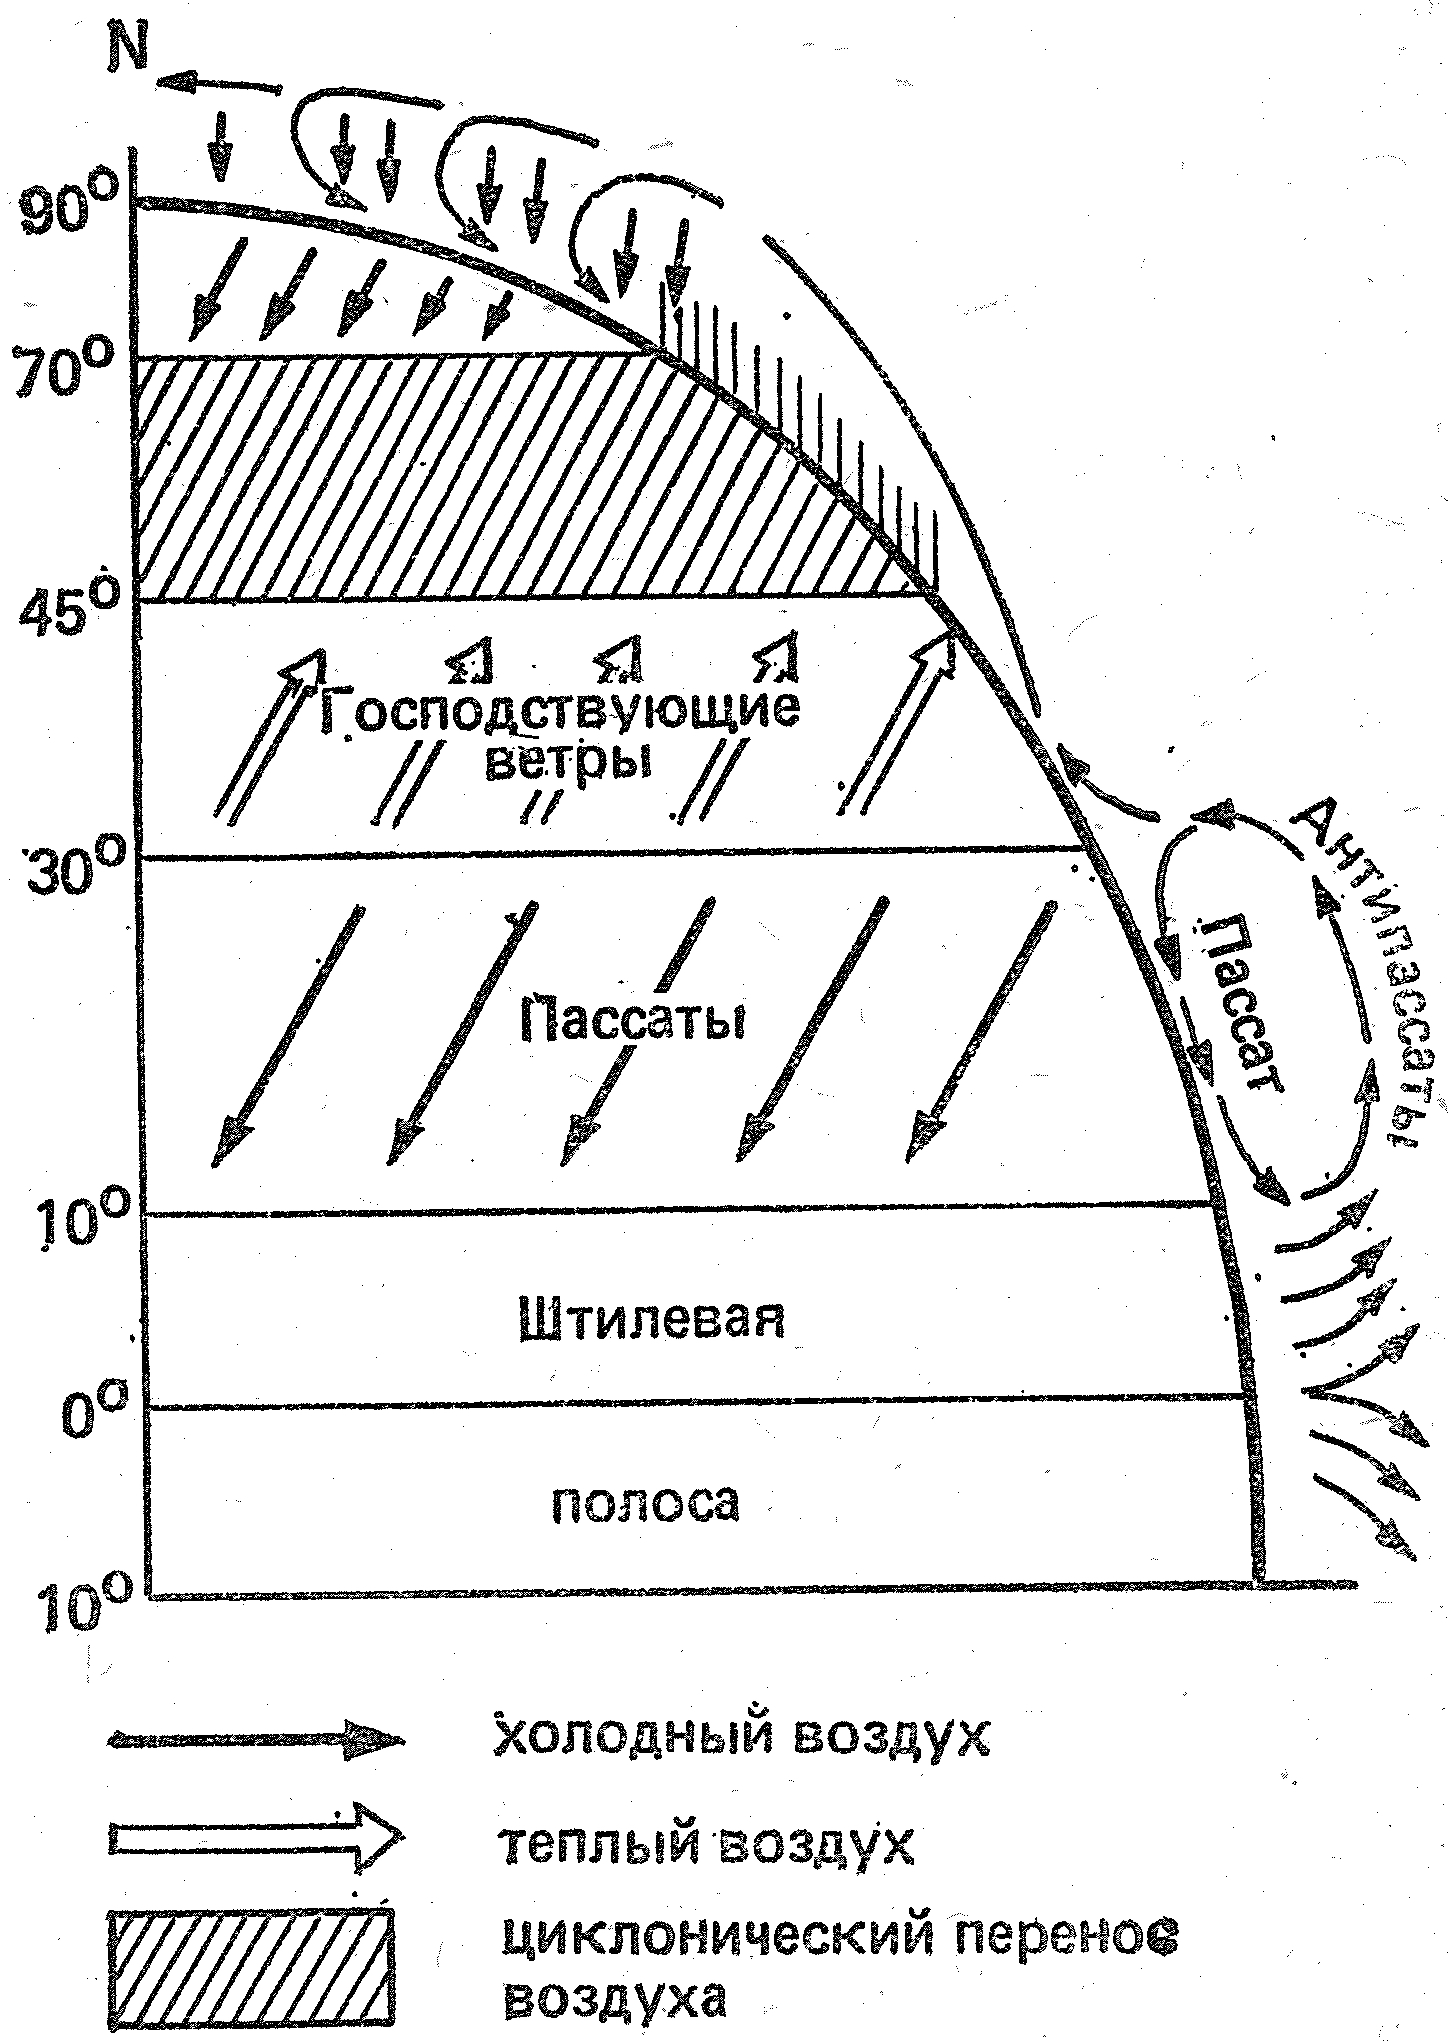
\includegraphics[scale=1.3]{0117P}
  \caption{Схема общей циркуляции атмосферы}
  \label{fig:117}
\end{figure*}

Как мы уже говорили, движение воздушных масс величина переменная и по скорости, и по направлению. Однако в масштабах глобальных это движение имеет четко выраженную закономерность, которая определяется общей циркуляцией атмосферы, зависящей от распределения атмосферного давления в обширных районах земного шара \--- от тропиков до Полярных зон. На схеме циркуляции воздуха между земной поверхностью и верхними слоями атмосферы (рис.~\ris{117}) видно, как вертикальные и горизонтальные потоки воздушных масс превращаются в ветры, имеющие постоянный сезонный характер.

В экваториальной зоне теплый воздух тропиков поднимается вверх, на границе тропосферы образуя ветер антипассат, растекающийся к северу и к югу.

Охлажденные воздушные массы \textbf{антипассата} оседают на поверхность земли, создавая в субтропиках повышенное давление и ветер, называемый уже \textbf{пассатом}, который устремляется в экваториальную зону.

Под действием силы Кориолиса пассаты северного полушария получают северо\-/восточное направление, а южного полушария (кроме северной части Индийского океана, где дуют сезонные муссонные ветры) \--- юго\-/восточное. Скорость пассатных ветров также постоянна и достигает 5\otdo 10~м/с.

В экваториальной зоне пассаты ослабевают и поворачивают на восток. Поэтому между пассатами обоих полушарий возникает штилевая зона (в Атлантике \--- <<конские широты>>), характерная пониженным давлением, грозами, ливнями и штилями.

В широтах 40\otdo 60\gr обоих полушарий преобладают ветры западной четверти. Они менее устойчивы (от $NW$ до $SW$), но значительно сильнее (10\otdo 15~м/с или 6\otdo 7 баллов). В южном полушарии, где западные ветры огибают весь Мировой океан, лежали основные пути парусных судов для плавания из Европы в Австралию и обратно в Европу вокруг мыса Доброй Надежды и мыса Горн. За свою силу и частые штормы (повторяемость до 50\,\%) эти ветры получили прозвище <<бравые весты>>, а широты \--- <<гремящие сороковые>> и <<ревущие шестидесятые>>.

В приполярных районах обоих полушарий, где оседают холодные массы воздуха верхних слоев тропосферы (при вертикальном температурном градиенте, падающем на 0,6\grC на каждые 110~м высоты.), образуя так называемые полярные максимумы, преобладают юго\-/восточные и восточные ветры.

Пассаты \--- первые в категории \textbf{господствующих ветров}, т.\=,е. постоянно дующих в определенных районах течение определенного промежутка времени. Скорость и направление господствующих ветров определяется многолетним наблюдениям для каждого моря или морского района.

Другая категория ветров \--- \textbf{местные}, дующие только в данном месте или нескольких местах земного шара возникают они при изменении тепловых условий в течение некоторое времени или под влиянием рельефа местности (характера подстилающей поверхности).

\begin{figure}[htb]
  \centering{}
  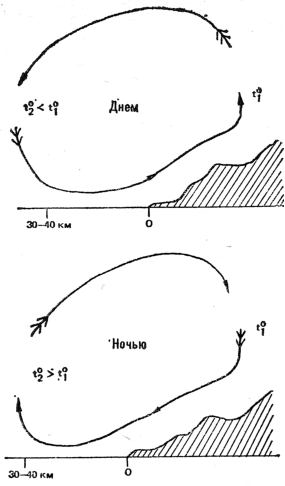
\includegraphics[scale=1.2]{0118P}
  \caption{Бризы}
  \label{fig:118}
\end{figure}

К первому типу относятся следующие ветры:
\begin{description}
\item [Бриз] \--- ветер, возникающий из неравномерного нагревания воды суши в прибрежной полосе моря (около 30\otdo 40~км). Морской бриз дует днем с моря на сушу и начинает около 10 часов утра, а береговой \--- суши на море и начинается после захода солнца. Ветер вертикально развития и на высоте нескольких с метров дует в обратном направлении (рис.~\ris{118}). Интенсивность бриза зависит от погоды. В жаркие летние дни морской бриз имеет умеренную силу до 4 баллов (4\otdo 7~м/с). Береговой бриз значительно слабее;
\item[Фен] \--- горячий сухой ветер, который возникает при обтекании влажно воздуха ветром горных вершин и нагревании его теплой подветренной подстилающей поверхностью горного склона. На Черном море наблюдает у побережья Крыма и Кавказа преимущественно весной.
\end{description}

Представителем второго типа местных ветров надо назвать прежде всего бору:
\begin{description}
\item[Бора] \--- очень сильный, порывистый и холодный ветер, направленный вниз по горному склону в местностях, где горный хребет граничит с теплым морем. Холодный воздух с большой скоростью устремляется вниз, к морю, достигая иногда силы урагана. В зимнее время, при низких температурах, вызывает обледенение. Наблюдается в районе Новороссийска, у берегов Далмации (Адриатическое море) и на Новой Земле;
\item[Бакинский норд] \--- холодный северный ветер в зоне Баку, дующий летом и зимой. Достигает штормовой, а нередко и ураганной силы (от 20 до 40~м/с). Приносит с берега тучи песка и пыли;
\item[Сирокко] \--- очень теплый и влажный ветер, зарождающийся в Африке и дующий в Центральной части Средиземного моря. Сопровождается облачностью и осадками.
\end{description}

Все сведения о господствующих и местных ветрах для данного моря (или морского района) даются в Лоциях.

\begin{figure}[htb]
  \centering{}
  \includegraphics[scale=1.2]{0119P}
  \caption{Муссоны}
  \label{fig:119}
\end{figure}

Существуют также сезонные ветры, называемые муссонами, которые носят континентальный характер и возникают вследствие разницы в атмосферном давлении при неравномерном нагревании суши и моря в летнее и зимнее время.

Как и другие ветры, муссоны имеют барический градиент, направленный в сторону низкого давления \--- летом на сушу, зимой на море (рис.~\ris{119}). Под влиянием силы Кориолиса в северном полушарии летние муссоны Тихого океана у восточного побережья Азии отклоняются к юго\-/востоку, а в Индийском океане \--- к юго\-/западу. Эти муссоны приносят с океана на Дальний Восток пасмурную, с дождями, моросью и туманами погоду, а на южное побережье Азии несут затяжные и обильные дожди, частые наводнения.

Зимние муссоны меняют направление на противоположное (120\gr\otdo 180\gr), и в Тихом океане они дуют уже с северо\-/запада, а в Индийском \--- с северо\-/востока в сторону океана. Скорость ветра в муссонах неравномерна. Зимние северо\-/восточные муссоны совпадают с пассатами северного полушария, и их скорость не превышает 5\otdo 10~м/с. Летние же муссоны Индийского океана достигают штормов силы. Смена муссонов происходит в апреле\--мае и октябре\--ноябре.

\begin{figure}[htb]
  \centering{}
  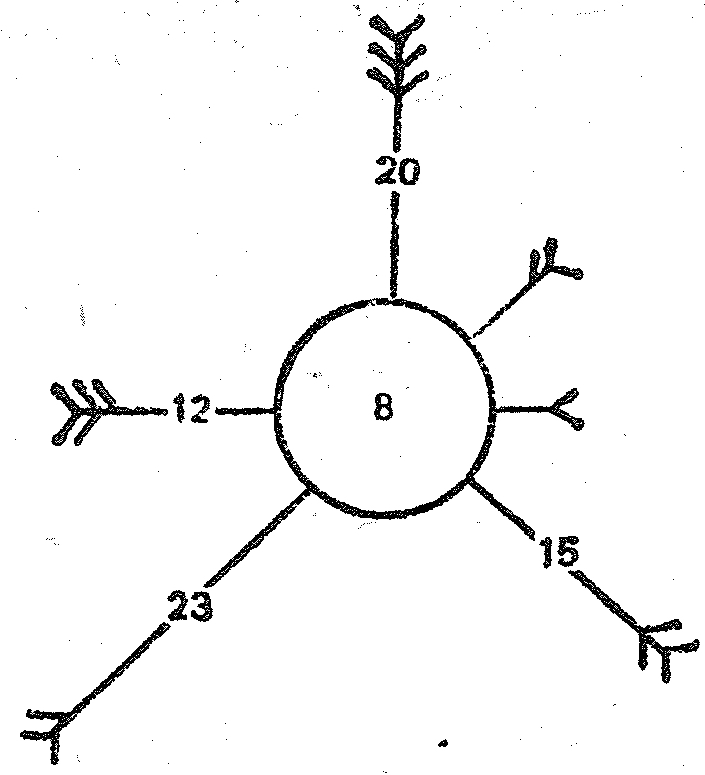
\includegraphics[scale=1.2]{0120P}
  \caption{Роза ветров}
  \label{fig:120}
\end{figure}

Ветер \--- основной движитель парусного судна. Поэтому с его направлением и силой приходится считаться в первую очередь. При выборе наиболее благоприятного маршрута для длительного крейсерского плавания полезно воспользоваться картой ветров, на которой поверхность моря или океана разбита на квадраты. В центре квадрата, внутри кружка, цифрами указывается повторяемость штилей. От центра кружка расходятся лучи по главным и четвертным румбам. Длина лучей пропорциональна повторяемости ветров этого направления, а на их концах наносится оперение, показывающее среднюю силу ветра. Если повторяемость ветра более 12\,\%, то на луче пишется величина повторяемости, если меньше 5\,\% \--- лучей не делают. Этот графический способ нанесения на карту ветровой обстановки на определенное время года, исчисленной на основании многолетних наблюдений, называется \textbf{розой ветров} (рис.~\ris{120}).

Изучая розы ветров, лежащие на пути яхты, капитан может оценить ветровую обстановку при проработке маршрута плавания.

\section{Погода}

Погодой называется физическое состояние атмосферы в данном месте, в данное время или в ограниченном промежутке времени (сутки, месяц, год).

Непрерывные изменения погоды зависят прежде всего от суточного и годового хода всех составляющих ее метеорологических элементов. Называют их \textbf{периодическими}, потому что они связаны с периодичностью движения Земли вокруг своей оси (суточное) и вокруг Солнца (годовое). Процессы же, происходящие при перемещении воздушных масс, вызывают \textbf{непериодические} изменения погоды. Изучение этих изменений и исследование процессов в границах общей циркуляции атмосферы с целью прогнозирования погоды \--- основная задача синоптической метеорологии. Воздушные массы, атмосферные фронты, циклоны и антициклоны, их возникновение, развитие, перемещение и взаимодействие \--- вот объекты наблюдений синоптиков.

\textbf{Воздушные массы.} Значительное количество в тропосфере воздуха, имеющего однородные физические свойства и простирающегося в горизонтальном направлении на тысячи километров и на 10\otdo 15 км по вертикали, называется воздушной массой.

Очаги формирования воздушной массы, где она приобретает определенные физические свойства, обычно находятся в области малоподвижных циклонов или антициклонов, над однообразной подстилающей поверхностью с однородным тепловым балансом \--- океанами, пустынями, степью, тундрой, Ледовитым океаном и т.\=,д.

Воздушные массы классифицируются по двум признакам: географическому \--- по положению очага формирования и термодинамическому \--- по температуре, полученной в очаге формирования.

\textbf{Географическая классификация воздушных масс.}

\begin{enumerate}
\item \begin{description}
  \item[Арктический (антарктический) воздух (АВ)] \--- формируется за северным и южным полярными кругами. Малозапыленная, очень устойчивая и прозрачная воздушная масса, с низкими температурами и большой относительной влажностью, создающей туманы и дымки. Может быть морским и континентальным.
  \item[Морской АВ (маВ)] \--- формируется в северном полушарии, в частности в Атлантическом океане, между Гренландией, Шпицбергеном и Кольским полуостровом. Увлажняясь над океаном, приносит в Европу холодную и пасмурную со снегом погоду зимой и похолодание с ливнями летом.
  \item[Континентальный АВ (каВ)] \--- формируется в северном полушарии в границах Европы, над Центральной Арктикой и приносит ясную и морозную погоду зимой, резкое похолодание \--- летом.
  \end{description}
\item \textbf{Полярный (ПВ) или умеренный (УВ) воздух} \--- формируется в умеренных широтах. Устойчивость его зависит от очага формирования и направления движения. Также может быть морским (мПВ) и континентальным (кПВ).
\item \textbf{Тропический воздух (ТВ)} \--- формируется в зоне субтропических антициклонов, сильно прогревается в очаге формирования. Морской тропический воздух (мТВ) характерен большой абсолютной влажностью и неустойчивостью, континентальный ТВ - большой неустойчивостью, жарой.
\item \textbf{Экваториальный воздух (ЭВ)} \--- рождается в экваториальной зоне, характерен резко выраженными свойствами тропического воздуха.
\end{enumerate}

\textbf{Термодинамическая классификация воздушных масс.}
\begin{enumerate}
\item \textbf{Холодная воздушная масса (ХМ)} перемещается из холодного в более теплый район. Процессы в такой массе, прогреваемой снизу, большей частью неустойчивы. Воздух характеризуется сильной конвективностью, турбулентностью и порывистыми ветрами. Холодным массам, особенно морского арктического или морского полярного воздуха, сопутствуют кучевые и кучево-дождевые облака, несущие ливневые осадки, грозы, шквалы. Над морем характерна в зимнее время.
\item \textbf{Теплая воздушная масса (ТМ)} двигается из теплого района в более холодный. Охлаждаясь снизу, она несет с собой моросящие осадки и адвективные туманы. Атмосферные процессы в ней обычно устойчивы. Над морем наблюдается летом.
\item \textbf{Местная воздушная масса (ММ)} длительное время находится в одной географической зоне, поэтому ее основные свойства изменяются мало, а температурный режим и устойчивость зависят от соседства с воздушной массой другого типа.
\end{enumerate}

\textbf{Атмосферные фронты.} При движении воздушные массы разных типов неизбежно соприкасаются друг с другом. Это сопровождается резким изменением погоды. Переходная зона между двумя массами называется поверхностью раздела, или фронтальной поверхностью, а линия пересечения этой поверхности с земной - атмосферным фронтом.

Если фронт образовался между основными географическими типами воздушных масс \--- АВ и ПВ, ПВ и ТВ, ТВ и ЭВ, он называется главным в отличие от вторичных (приземных) фронтов, образующихся между географическими однородными воздушными массами.

\begin{figure*}[htb]
  \centering{}
  \includegraphics[scale=1.3]{0121P}
  \caption{Теплый фронт}
  \label{fig:121}
\end{figure*}

\textbf{Теплый фронт} возникает при наползании теплой воздушной массы на холодную (рис.~\ris{121}). Теплые массы, поднимаясь наклонно вверх, адиабатически (адиабатически \--- без притока тепла извне или отдачи его в окружающую среду) охлаждаются \--- возникает широкая пелена облаков слоистых форм с зоной обложных осадков впереди фронта. Давление перед фронтом падает. Предшественниками теплого фронта являются перистые облака в виде <<коготков>>. Судно, пересекая зону теплого фронта, попадает в широкую полосу обложного дождя или снега с пониженной видимостью. Перед теплым фронтом наблюдаются так называемые предфронтальные туманы.

\begin{figure*}[htb]
  \centering{}
  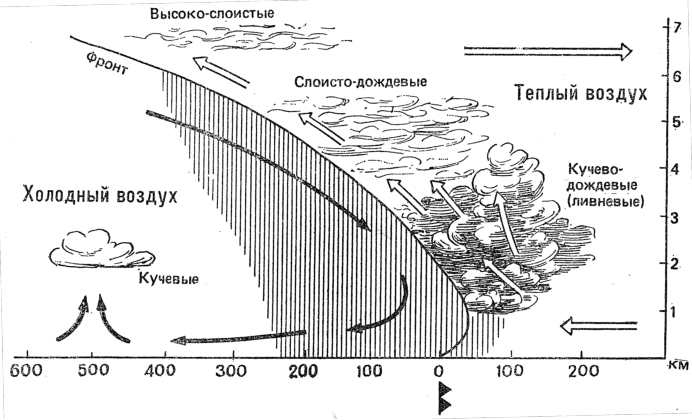
\includegraphics[scale=1.3]{0122P}
  \caption{Холодный фронт}
  \label{fig:122}
\end{figure*}

\textbf{Холодный фронт второго рода} движется быстро и возникает при энергичном <<подклинивании>> холодных масс под теплые, которые выжимаются вверх. В результате адиабатического охлаждения в них образуются кучево\-/дождевые облака, сопровождаемые ливнями и грозами. Холодный фронт с ливневыми облаками наступает <<стеной>>. Впереди, в качестве предвестников фронта, быстро движутся перисто\-/кучевые облака; ниже, в среднем ярусе, продвигаются <<обточенные>> ветром высококучевые чечевицеобразные.

Давление непосредственно перед фронтом сильно и неравномерно падает, судно попадает в зону ливней, гроз, шквалов и сильного волнения.

\textbf{Холодный фронт первого} рода движется медленнее по сравнению с холодным фронтом второго рода.

Клин холодного воздуха как бы подсекает теплые массы, вынуждая их подниматься вверх, что приводит к образованию облачной системы. Все процессы выражены не так бурно, как у холодного фронта второго рода. За линией фронта имеется пелена слоисто\-/дождевых и высокослоистых облаков, из которых выпадают обложные осадки (рис.~\ris{122}).

В результате слияния теплого и холодного фронтов возникает сложный фронт \--- фронт окклюзии. Скорость перемещения холодного фронта больше, чем теплого. Поэтому при слиянии фронтов теплый воздух вытесняется вверх, образуя верхний фронт.

В зависимости от соотношения температур характер фронта окклюзии может быть:
\begin{description}
\item[нейтрального типа] \--- вытесненные теплые массы и облачные системы фронтов располагаются по фронтальным поверхностям, а температуры холодных масс, догоняющей и уходящей, одинаковы. При этом осадки постепенно ослабевают и прекращаются; 
\item[теплого типа] \--- температура массы наступающего холодного фронта выше температуры лежащей впереди массы. Поэтому более теплая наступающая масса начинает "скользить" вперед и вверх по поверхности раздела теплого фронта; 
\item[холодного типа] \--- температура наступающего холодного фронта более низкая. Холодные массы начинают как бы подсекать более теплые и заставляют их восходить вдоль поверхности раздела холодного фронта. 
\end{description}

\begin{figure}[htb]
  \centering{}
  \includegraphics[scale=1.2]{0123P}
  \caption{Схема окклюдированного циклона}
  \label{fig:123}
\end{figure}

Погода окклюдированного фронта теплого типа сходна с погодой главных тепловых фронтов, а холодного типа \--- с погодой холодных фронтов.

\textbf{Циклоны и антициклоны.} Циклон и антициклон мы рассматривали как барические области низкого и высокого давления. Эти же области несут также и одну из форм циркуляции атмосферы \--- вихреобразные воздушные возмущения. В циклонах северного полушария эти вихри движутся по спирали против часовой стрелки, в южном \--- по часовой, но всегда направлены к центру циклона. Скорость ветра при этом всегда высокая. Так, в циклонах умеренных широт она достигает 20\otdo 30~м/с, т.\=,е. штормовой и ураганной силы, а в тропических циклонах нередко превышает 60\otdo 70~м/с.

Погода в циклонах, особенно на линии теплого фронта, всегда пасмурная, облачная и прохладная, летом \--- дождливая, а зимой \--- снежная с оттепелями. В теплом секторе молодого циклона облачности и осадков нет, но над морем может быть и пасмурно.

Развитие циклона проходит несколько стадий: волны, молодого циклона, окклюдированного циклона и заполненного циклона. На рис.~\ris{123} показана схема окклюдированного циклона северного полушария.

В отличие от циклонов в антициклонах спиральные вихревые возмущения направлены от центра антициклона. Ветровые потоки в северном полушарии дуют по часовой стрелке, в южном \--- против часовой стрелки.

Погода в антициклоне обусловлена оседанием воздушных масс, их адиабатическим сжатием и как следствие повышением температуры воздуха. Поэтому летом она спокойная, характерна штилями и слабыми ветрами, малооблачностью и безоблачностью, с резким суточным ходом метеоэлементов. Зимой погода ясная и морозная.

\textbf{Карты погоды} (синоптические карты) составляют по наблюдениям метеоэлементов на метеорологических станциях в установленное (стандартное) время.

Для основных (приземных) синоптических карт результаты наблюдений снимают в 0, 6, 8 и 18 часов по Гринвичу. Раскодированную радиоинформацию, полученную от береговых или судовых метеостанций, по определенной схеме условными знаками наносят на специальную карту. Для яхтенного капитана, обычно не имеющего избытка информации о погоде, очень важно уметь определять ожидаемую погоду по местным признакам.

\section{Прогноз погоды по местным признакам}

\begin{enumerate}
\item Ухудшение погоды (приближение циклона с теплым фронтом: приближение ненастной погоды, влажной, с осадками, свежим ветром через 6\otdo 12~ч):
  \begin{itemize}
  \item Атмосферное давление постепенно понижается при отсутствии суточного хода.
  \item Нарушается суточный ход температуры воздуха, влажности и ветра.
  \item Появляются быстро движущиеся от горизонта к зениту перистые когтевидные облака, которые постепенно сменяются перисто\-/слоистыми, переходящими в более плотный слой высокослоистых облаков.
  \item Перистые и перисто\-/слоистые облака движутся вправо от направления наземного ветра.
  \item Повышенная видимость, увеличение рефракции \--- появление предметов из-за горизонта.
  \item Усиление волнения, зыбь и волна начинают идти не по ветру.
  \item Повышенная слышимость в воздухе.
  \item Появление <<гало>> и венцов малых размеров.
  \item Сильное мерцание звезд ночью.
  \item Утренняя заря ярко\-/красной окраски.
  \item Ночью и утром нет росы.
  \item Движение облаков нижнего и верхнего ярусов в разных направлениях.
  \item Появляются ложные солнца, миражи и т.\=,п.
  \item Вечером солнце заходит в сгущающиеся плотные облака.
  \end{itemize}
\item Ухудшение погоды (приближение холодного фронта, грозы и шторма за 1\otdo 2~ч до его начала).
  \begin{itemize}
  \item Резкое падение атмосферного давления.
  \item Появление перисто\-/кучевых облаков.
  \item Появление плотных разорванных перистых облаков.
  \item Появление высококучевых, башеннообразных и чечевицеобразных облаков.
  \item Неустойчивость ветра.
  \item Появление сильных помех в радиоприеме.
  \item Появление в море характерного шума со стороны приближения грозы или шквала.
  \item Резкое развитие кучево\-/дождевой облачности.
  \end{itemize}
\item Сохраняется плохая погода (пасмурная с осадками, сильным ветром, плохой видимостью) на ближайшие 6 или более часов.
  \begin{itemize}
  \item Низкое или понижающееся атмосферное давление не имеет суточного хода.
  \item Характер облачности (слоисто\-/дождевые, кучево\-/дождевые облака) не меняется.
  \item Температура воздуха летом пониженная, зимой повышенная, не имеет суточного хода.
  \item Ветер свежий, не меняет своей силы, характера и мало меняет направление.
  \end{itemize}
\item Улучшение погоды (после прохождения теплого фронта или фронта окклюзии можно ожидать прекращения осадков и ослабления ветра в ближайшие 4~ч).
  \begin{itemize}
  \item Падение давления прекращается, барометрическая тенденция становится положительной.
  \item Появление просветов в облаках. Высота облаков увеличивается. Слоисто\-/дождевые облака сменяются слоисто\-/кучевыми и слоистыми.
  \item Ветер поворачивает вправо и ослабевает.
  \item Волнение моря начинает успокаиваться.
  \item Местами на море появляется туман (при температуре воды ниже температуры воздуха).
  \end{itemize}
\item Улучшение погоды (после прохождения холодного фронта второго рода можно ожидать прекращения осадков, изменения направления ветра и прояснения через 2\otdo 4~ч).
  \begin{itemize}
  \item Резкий рост атмосферного давления.
  \item Резкий поворот ветра вправо.
  \item Резкое изменение характера облачности, увеличение просветов.
  \item Резкое увеличение видимости.
  \item Понижение температуры.
  \item Ослабление помех в радиоприеме.
  \end{itemize}
\item Сохраняется хорошая антициклоническая погода (с тихим ветром или штилем, ясным небом или небольшой облачностью и хорошей видимостью) в течение ближайших 12~ч:
  \begin{itemize}
  \item Высокое атмосферное давление имеет суточный ход.
  \item Температура воздуха с утра низкая, к 15~ч повышается, а к ночи понижается.
  \item Ветер к ночи или к рассвету затихает, к 14~ч усиливается; до полудня поворачивает по солнцу, после полудня \--- против солнца.
  \item В прибрежной полосе наблюдаются правильно сменяющиеся утренние и вечерние бризы.
  \item Появление по утрам отдельных перистых облаков, исчезающих к полудню.
  \item Ночью и утром роса на палубе и других предметах.
  \item Золотистые и розовые оттенки зари, серебристое сияние на небе.
  \item Сухая мгла у горизонта.
  \item Образование наземного тумана по ночам и утрам и исчезновение после восхода солнца.
  \item Солнце опускается на чистый горизонт.
  \end{itemize}
\item Характер погоды сохраняется на ближайшее время.
  \begin{itemize}
  \item Повторение в сроки наблюдений метеоэлементов прошедшего дня.
  \item Вид облачности, видимость, характер осадков, цвет неба, окраска зари, слышимость радиоприема, состояние моря, тип и характер волнения, оптические явления в атмосфере похожи на такие же признаки прошедшего дня.
  \end{itemize}
\end{enumerate}

В заключение уместно вспомнить некоторые мнемонические морские поговорки, которые облегчали морякам борьбу с морской стихией в давние времена, когда каждый капитан <<был сам себе бюро погоды>>.

\begin{multicols}{2}

\small

\begin{quote}
Ходят чайки по песку \\*
Моряку сулят тоску. \\*
И пока не сядут в воду, \\*
Штормовую жди погоду.
\end{quote}

\begin{quote}
Барашки по небу бегут, \\*
Иль небо метлами метут, \\*
Когда рангоут твой высок, \\*
Оставь лишь марсели да фок!
\end{quote}

\begin{quote}
Лезет стрелка вверх упорно, \\*
Не желая отдохнуть, \\*
Можешь ждать тогда бесспорно, \\*
Что от ОСТа будет дуть!\footnote{Для северного полушария}
\end{quote}

\begin{quote}
При низком барометре \--- первый подъем, \\*
Шквалов здоровых, бесспорно, мы ждем.
\end{quote}

\begin{quote}
Если стрелка вдруг упала. \\*
Жди грозы, дождя иль шквала; \\*
Если ж стрелка поднимается, \\*
То погода улучшается.
\end{quote}

\begin{quote}
Скачет стрелка вверх и вниз \\*
То погоды лишь каприз \\*
Если ж медленно движенье \--- \\*
Жди надолго измененья.
\end{quote}

\begin{quote}
Если тучи громоздятся \\*
В виде башен или скал, \\*
Скоро ливнем разразятся, \\*
Налетит жестокий шквал.
\end{quote}

\begin{quote}
Если сгрудятся тучи и быстро летят, \\*
Скоро все снасти твои затрещат. \\*
Если на клочья начнут они рваться \--- \\*
Ставь брамселя: их не стоит бояться!
\end{quote}

\begin{quote}
Вечером небо коль полно огня, \\*
Утром же зорю туман застилает \\*
Верные признаки ясного дня, \\*
Старый моряк парусов прибавляет.
\end{quote}

\begin{quote}
Птицы коль к берегу держат свой путь \--- \\*
Ветер здоровый, поверь, будет дуть!
\end{quote}

\begin{quote}
Дождик раньше, ветер вслед \--- \\*
Жди от шквала всяких бед! \\*
После ветра дождь придет \--- \\*
Значит, скоро шквал пройдет.
\end{quote}

\begin{quote}
Если солнце село в воду \--- \\*
Жди хорошую погоду, \\*
А когда садится в тучу \--- \\*
Берегись, получишь бучу!
\end{quote}

\normalsize

\end{multicols}

Разумеется, местные признаки погоды помогают яхтенному капитану, если он хорошо изучил природу и физическую сущность атмосферных явлений и процессов.

\section{Элементы океанологии}

В спортивном мореплавании на больший интерес представляет динамика моря \--- его волнение, морские течения, приливы и отливы.

\textbf{Волнение.} Морские волны вызываются колебательными движениями частичек воды под действием какой\-/либо внешней силы \--- ветра, прилива, подводного землетрясения (цунами), изменения атмосферного давления (барические волны, или сейши), движения судна. Чаще всего плавающее судно испытывает действие ветрового волнения и в приливных зонах \--- приливной и отливной волны.

\begin{figure}[htb]
  \centering{}
  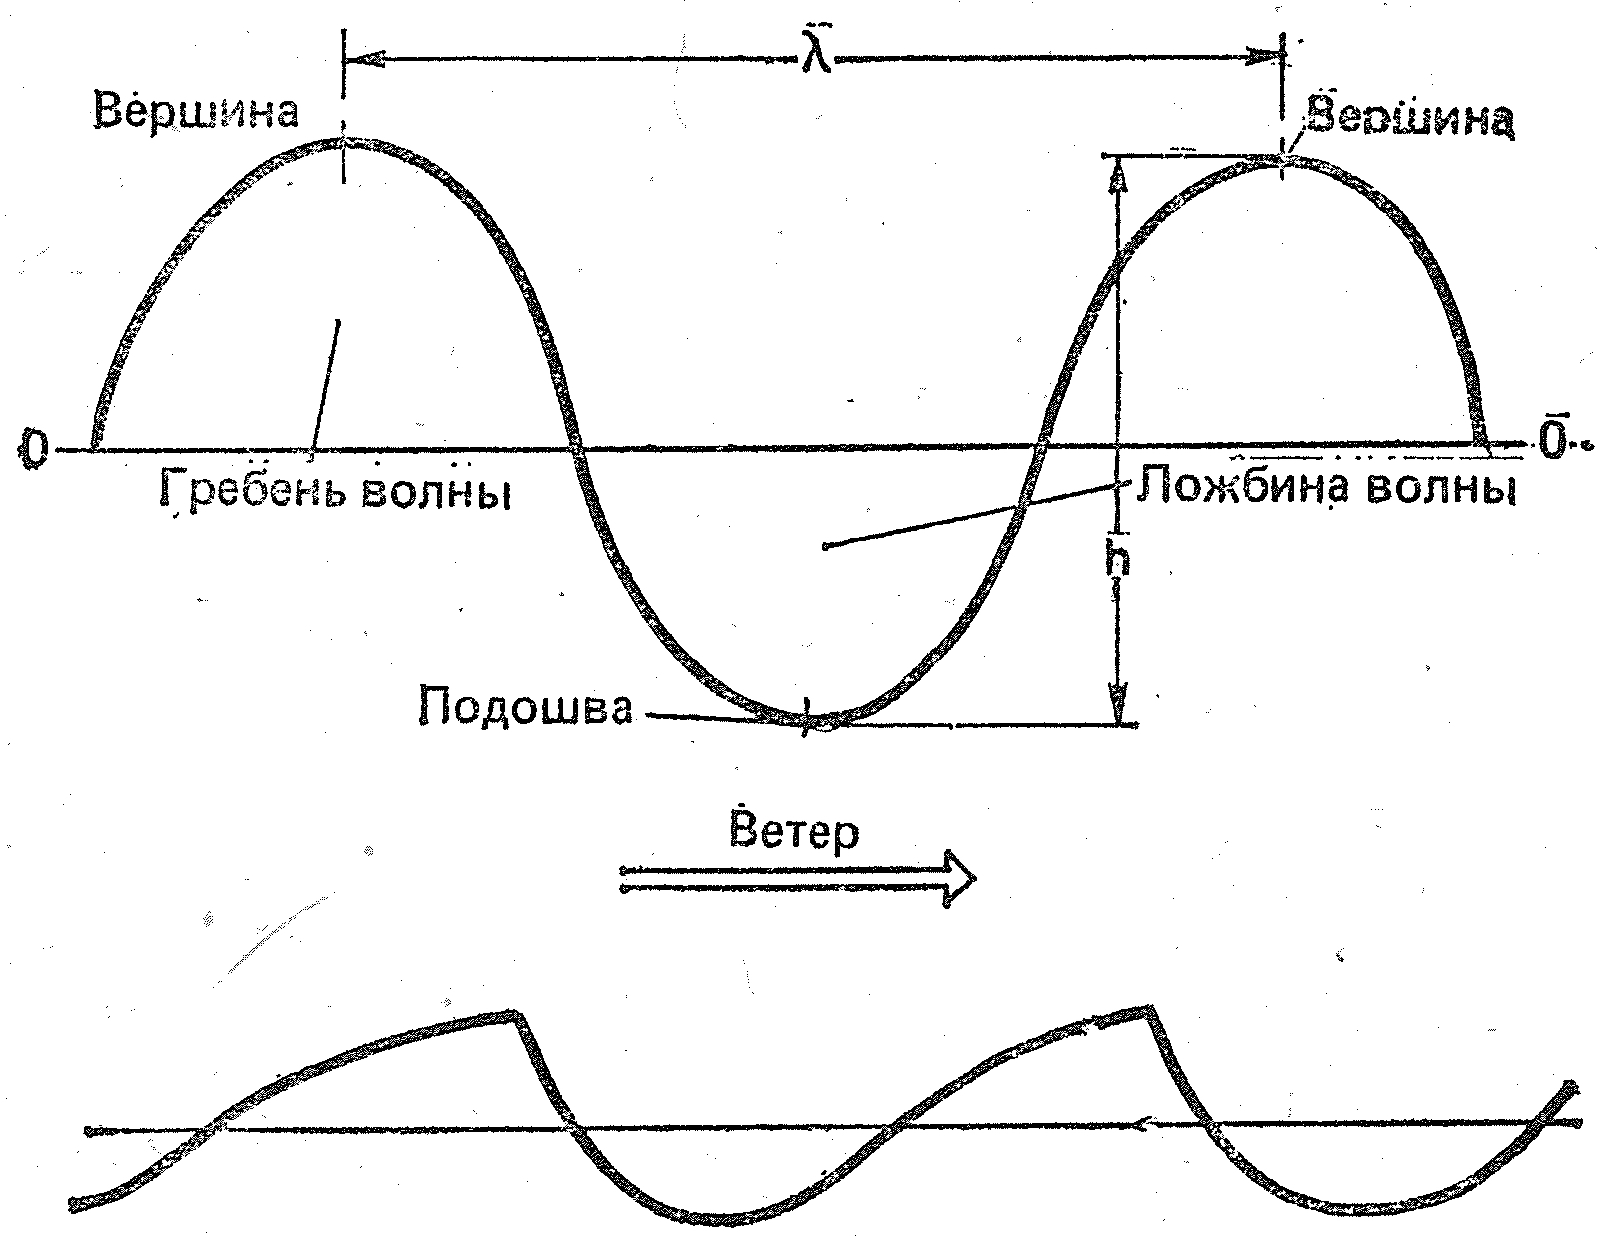
\includegraphics[scale=1.2]{0124P}
  \caption{Элементы волны и форма ветровой волны}
  \label{fig:124}
\end{figure}

Любая волна имеет следующие элементы (рис.~\ris{124}):
\begin{description}
\item[гребень] \--- часть волны, расположенная выше спокойного уровня;
\item[вершина] \--- наивысшая точка гребня;
\item[ложбина] \--- часть волны, расположенная ниже спокойного уровня;
\item[подошва] \--- наивысшая точка ложбины волны.
\end{description}

Кроме того, каждую конкретную волну характеризуют элементы, имеющие численное выражение:
\begin{description}
\item[высота (h)] \--- расстояние по вертикали от подошвы до вершины волны;
\item[длина ($\lambda$)] \--- горизонтальное расстояние между вершинами двух смежных гребней;
\item[крутизна] \--- отношение высоты волны к ее длине ($k = h / \lambda$);
\item[период ($\tau$)] \--- промежуток времени, за который волна проходит свою длину;
\item[скорость распространения ($c$)] \--- расстояние, проходимое вершиной волны в единицу времени;
\item[направление распространения ($N\gr$)] \--- угол, отсчитываемый по картушке компаса от $N$ (или истинный румб, откуда движутся волны).
\end{description}

Линия, проходящая вдоль гребня данной волны, называется \textbf{фронтом}, а линия, перпендикулярная фронту \--- \textbf{волновым лучом}.

Ветровое волнение \--- результат непосредственного действия ветра на воду в данном месте в данный момент. Ветер изменяет форму волны, которая отличается тем, что подветренная ее сторона значительно круче наветренной (см. рис.~\ris{124}). Под действием ветра начинается поверхностное движение воды под ветер, гребень волны опережает нижележащие частицы воды и рассыпается, образуя пенистые барашки.

Крутизна волны зависит от глубины места: чем меньше глубина, тем круче волны, тем быстрее они разрушаются, образуя прибои (у берега) и буруны (на мелководье или на рифах), предупреждая тем самым об опасности.

Высота волны зависит от силы ветра: океанская штормовая волна достигает 8~м, а ураганная \--- 15\otdo 20~м при длине до 400~м (на внутренних морях \--- 5 м при длине 20\otdo 40~м). Однако в силу вязкости воды высота волны имеет предел, после которого она не увеличивается, какой бы силы ни дул ветер.

На водохранилищах при сильных ветрах волны имеют большую крутизну при высоте 2~м и более.

Волнение успокаивается, если на поверхности воды находятся водоросли, битый лед или <<сало>>, а также при сильном дожде.

Направления волнения и ветра обычно совпадают, но в некоторых случаях они могут и разниться до четырех румбов.

Волнение, которое по инерции возникает после прекращения ветра, называется зыбью. В этом случае волны приобретают правильную симметричную форму и отличаются большой длиной с очень малой крутизной. Зыбь в штилевую погоду называется мертвой зыбью. Обычно она может служить признаком надвигающегося шторма или сильного ветра, проходящего стороной.

При встрече волн разных направлений (например, зыби и волны от ветра другого направления) или отражении волн от стен гидротехнических сооружений (волноломов, пирсов и т.\=,д.) возникает толчея \--- беспорядочные стоячие волны. На толчее в сильный ветер малыми судами, особенно тихоходными, управлять плохо, и это надо иметь в виду при подходе к стенке.

Влияние волнения, особенно штормового, однозначно: оно не только нарушает нормальный ритм жизни и работы, но в ряде случаев представляет прямую опасность. Штормовая качка приводит к перенапряжению всех связей корпуса, особенно деревянного, рангоута и такелажа. Яхта, попавшая в шторм на мелководье, рискует на большой волне потерять фальшкиль. Поэтому никакие меры безопасности в штормовых условиях никогда не будут чрезмерными.

\begin{figure}[htb]
  \centering{}
  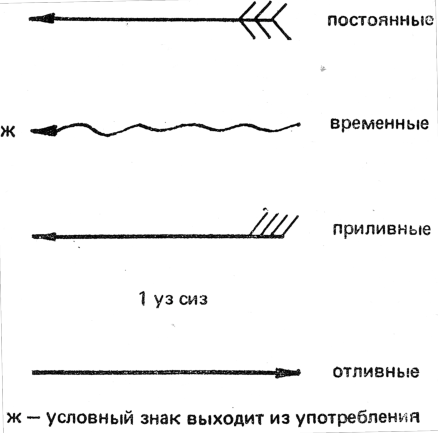
\includegraphics[scale=1.2]{0125P}
  \caption{Условные знаки течения на карте}
  \label{fig:125}
\end{figure}

\textbf{Морские течения.} Морское течение \--- поступательное перемещение больших масс воды \--- представляет практическое значение в мореплавании. Обладая направлением и скоростью, оно оказывает прямое воздействие на направление движения и скорость судна. В этом смысле важную роль играют ветровые (дрейфовые), поверхностные и приливо-отливные течения.

Ветровые течения могут быть постоянными в районах господствующих ветров, чьи скорость и направление меняются мало, и временными (непериодическими), возникающими при кратковременном действии ветра. Скорость ветрового течения зависит от силы ветра: 0,5\otdo 0,7 (ветер около 5\otdo 6~баллов) \--- 1,0~уз (в шторм).

\textbf{Поверхностные (навигационные) течения} наблюдаются на глубинах до 15~м от уровня моря, но могут распространяться и глубже. Они также бывают постоянными (в океанах \--- Гольфстрим, Куросиво) и временными. Скорости постоянных течений различны. Они указываются на навигационных картах и в Лоциях (рис.~\ris{125}).

В плавании все течения учитываются навигационными способами.

\begin{figure}[htb]
  \centering{}
  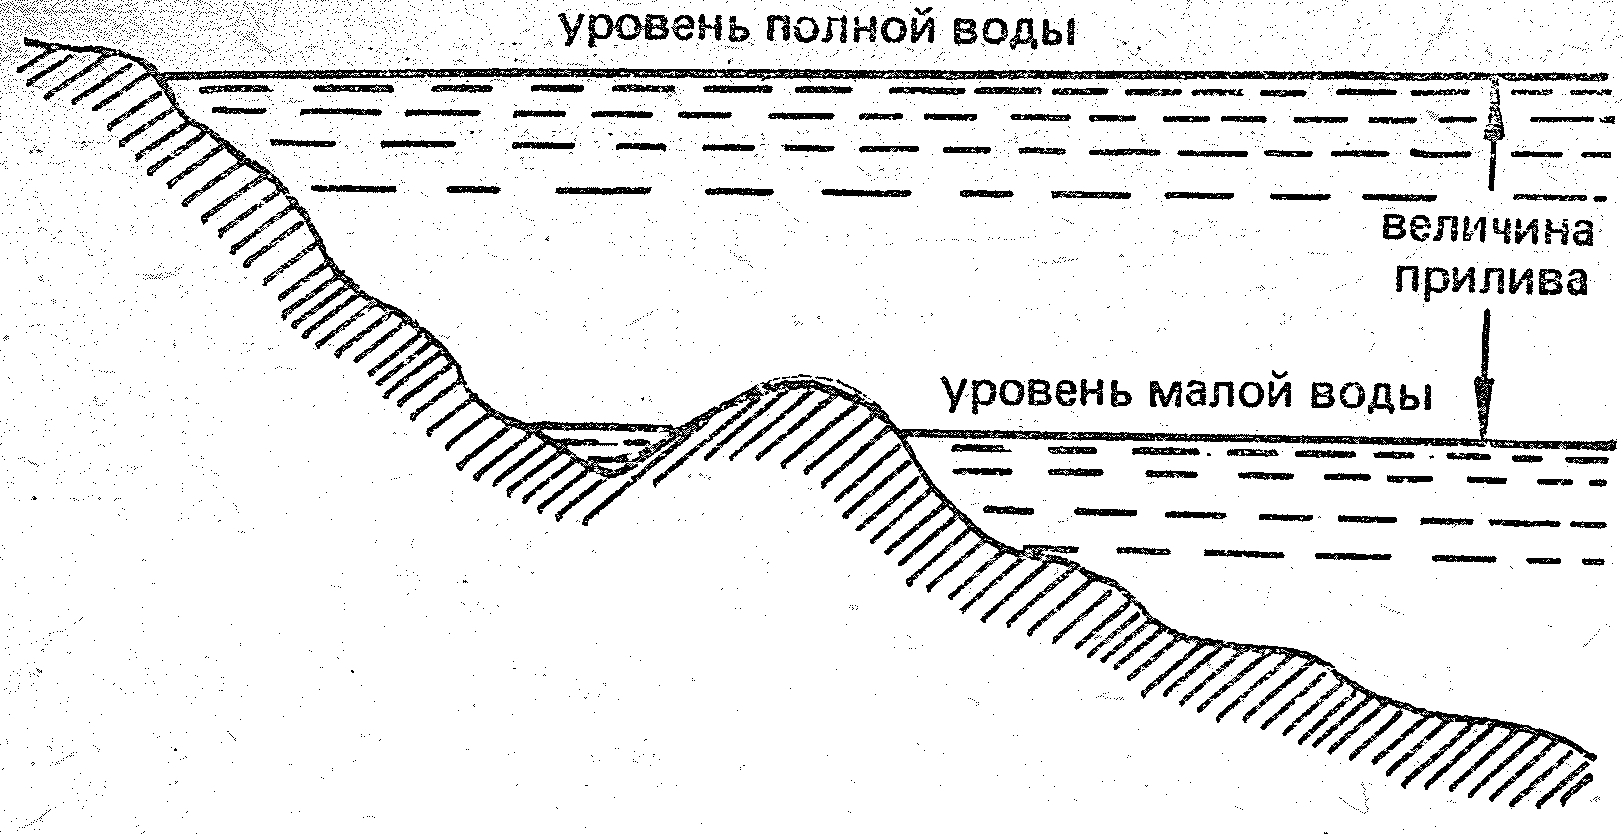
\includegraphics[scale=1.2]{0126P}
  \caption{Уровни и величина прилива}
  \label{fig:126}
\end{figure}

\textbf{Приливы и отливы} \--- периодические колебания водных масс \--- заключаются в постепенном повышении уровня воды до наивысшего и затем постепенным их понижением до самого низкого (рис.~\ris{126}). Максимальный уровень воды называется \textbf{полной водой}, минимальный, после отлива, \--- \textbf{малой водой}. Разность между этими уровнями в одном периоде называют \textbf{величиной прилива}.

Это явление возникает под влиянием приливообразующих сил, чья природа лежит во взаимном притяжении Земли, Луны и Солнца. Они влияют на подвижную водную оболочку нашей планеты. В значительной степени на приливы влияет притяжение Луны, расположенной намного ближе к Земле, чем Солнце. Поэтому сила лунных приливов больше чем в 2 раза силы солнечных. И хотя эти приливы независимы друг от друга, но, складываясь, они образуют единый лунно\-/солнечный прилив.

\begin{figure}[htb]
  \centering{}
  \includegraphics[scale=1.2]{0127P}
  \caption{Фазовое неравенство приливов}
  \label{fig:127}
\end{figure}

При вращении вокруг Земли Луна в течение лунного месяца последовательно проходит через четыре фазы (рис.~\ris{127}). На рисунке видно, что при полнолунии и новолунии приливообразующие силы совпадают и вызывают максимальные (сизигийные) приливы. Когда же Луна находится в первой или последней четверти, приливообразующие силы делятся и возникают минимальные (квадратурные) приливы. Такое неравенство приливов называют фазовым, или полумесячным. Период изменений приливов равен 14,6~суток.

Различают три формы приливов: суточные, имеющие в период лунных суток (\hhmm{24}{50}) одну полную воду и одну малую; полусуточные, у которых за это же время сменяются две полные воды и две малые; смешанные \--- с переменой в течение половины лунного месяца периодов с полусуточных на суточный, и наоборот.

Наибольшие величины приливов наблюдаются в Атлантическом океане \--- 18~м (о.~Фанди), 11\otdo 12~м (у побережья Англии). В Тихом океане они меньше \--- 7\otdo 8~м (у Аляски) и 13~м (в Охотском море).

Основным пособием по приливам для мореплавателя являются <<Таблицы приливов>>. Они бывают постоянные и ежегодные. Постоянные <<Таблицы>> состоят из трех книг: <<Воды Европейской части СССР и прилегающих к ним зарубежных районов>>, <<Воды Азиатской части СССР>> и <<Зарубежные воды>>. В ежегодных <<Таблицах>> зарубежные воды представлены двумя книгами: <<Атлантический, Индийский и Северный Ледовитый океан>> и <<Тихий океан>>.

С помощью этих <<Таблиц>> можно вычислить:
\begin{itemize}
\item высоты и моменты полных и малых вод в основных портах на заданные сутки; 
\item высоты уровня моря в основном порту на любой заданный момент между полной и малой водой; 
\item время, когда прилив достигает заданной величины. 
\end{itemize}

При пользовании <<Таблицами приливов>> следует внимательно ознакомиться с оглавлением книги и пояснениями к ней.
Приливам всегда сопутствуют приливо\-/отливные течения \--- периодические поступательно\-/возвратные движения водных масс, которые зависят в основном от характера прилива.

Скорости приливо\-/отливных течений в разных бассейнах не одинаковы и могут быть от 1\otdo 5 (в Белом море) до 0,1\otdo 8~уз и более (в Тихом океане). Кроме того, приливы активно участвуют в изменении уровня воды. Это явление сложное и вызывается также сгонно\-/нагонными ветровыми течениями (классический пример \--- подобные течения в Финском заливе) и силами гравитации, стремящимися привести частицы воды в состояние покоя. При плавании крейсерских яхт с большой осадкой необходимо учитывать эти колебания.
